%Dokumentinformationen
\newcommand{\titleinfo}{Lineare Algebra - Formelsammlung}
\newcommand{\authorinfo}{N. Selvarajah, S.Walker, weitere HSR-Studenten}
\newcommand{\versioninfo}{HS 2018}
\newcommand{\licence}{CC BY-NC-SA}

%weitere Autoren: ==========================================================================
% N. Selvarajah, S.Walker, C.Gwerder, S.K\"orner, M.Ehrler, L. Leuenberger



% standard header
%Schriftgr"osse, Layout, Papierformat, Art des Dokumentes
\documentclass[10pt,twoside,a4paper,fleqn]{article}
%Einstellungen der Seitenr"ander
\usepackage[left=1cm,right=1cm,top=1cm,bottom=1cm,includeheadfoot]{geometry}
% Sprache, Zeichensatz, packages
\usepackage[utf8]{inputenc}
\usepackage[ngerman]{babel,varioref}
\usepackage{amssymb,amsmath,fancybox,graphicx,color,lastpage,wrapfig,fancyhdr,hyperref,verbatim,tabularx, textcomp}
%Text Umkreisung
\usepackage{tikz}
%Verweise auf anderes Kapitel
\usepackage{xr}
%\usepackage{hyperref} 

%pdf info
\hypersetup{pdfauthor={\authorinfo},pdftitle={\titleinfo},colorlinks=false}
%linkbordercolor=white
\author{\authorinfo}
\title{\titleinfo}

%Kopf- und Fusszeile
\pagestyle{fancy}
\fancyhf{}
%Linien oben und unten
\renewcommand{\headrulewidth}{0.5pt} 
\renewcommand{\footrulewidth}{0.5pt}

%Kopfzeile
\fancyhead[L]{\titleinfo{ }\tiny{(\versioninfo)}}
\fancyhead[R]{Seite \thepage { }von \pageref{LastPage}}

%Fusszeile
\fancyfoot[L]{\footnotesize{\authorinfo}}
\fancyfoot[C]{\footnotesize{\licence \quad $\rightarrow$ \href{https://github.com/HSR-Stud}{Github: HSR-Stud}}}
\fancyfoot[R]{\footnotesize{\today}}

%Neue Befehle:
%1: Fügt vertikaln Balken bei matrix ein.
%2: Umkreist den Text darin.
\makeatletter
\renewcommand*\env@matrix[1][*\c@MaxMatrixCols c]{%
	\hskip -\arraycolsep
	\let\@ifnextchar\new@ifnextchar
	\array{#1}}
\makeatother

\makeatletter
\newcommand*{\addFileDependency}[1]{% argument=file name and extension
	\typeout{(#1)}
	\@addtofilelist{#1}
	\IfFileExists{#1}{}{\typeout{No file #1.}}
}
\makeatother

\newcommand*{\myexternaldocument}[1]{%
	\externaldocument{#1}%
	\addFileDependency{#1.tex}%
	\addFileDependency{#1.aux}%
}

\newcommand*\circledr[1]	{
	\tikz [baseline = (char.base)]	{
		\node [shape = circle, draw = red, inner sep = 2pt, text = black] (char) {#1};
}
}

\newcommand*\circledb[1]	{
	\tikz [baseline = (char.base)]	{
		\node [shape = circle, draw = blue, inner sep = 2pt, text = black] (char) {#1};
}
}

\newcommand*\circledy[1]	{
	\tikz [baseline = (char.base)]	{
		\node [shape = circle, draw = orange, inner sep = 2pt, text = black] (char) {#1};
}
} 

\usepackage{multicol}
\usepackage{rotating}

%%%%%%%%%%%%%%%%%%%%%%%%%%%%%%%%%%%%%%%%%%%%%%%%%%%%%%%%%%%%%%%%%%%%%%%%%%%%%%%%%%%%%%%%%%%%%%%%
% Neue Befehle und Definitionen                
%%%%%%%%%%%%%%%%%%%%%%%%%%%%%%%%%%%%%%%%%%%%%%%%%%%%%%%%%%%%%%%%%%%%%%%%%%%%%%%%%%%%%%%%%%%%%%%%
\definecolor{black}{rgb}{0,0,0}
\definecolor{red}{rgb}{1,0,0}
\definecolor{white}{rgb}{1,1,1}
\definecolor{grey}{rgb}{0.8,0.8,0.8}
\newcommand{\formelbuch}[1]{$_{\textcolor{red}{\mbox{\small{S#1}}}}$}
\newcommand{\verweis}[2]{\small{(siehe auch \ref{#1}, #2 (S. \pageref{#1}))}}
\newcommand{\vektor}[3]{\left(\begin{array}{r} #1 \\ #2 \\ #3 \\ \end{array}\right)}

\newcommand\kariert[2][0.5cm]{% 
	\begin{tikzpicture}[gray,step=#1]
	\pgfmathtruncatemacro\anzahl{(\linewidth-\pgflinewidth)/#1} % maximale Anzahl Kästchen pro Zeile
	\draw (0,0) rectangle (\anzahl*#1,#2*#1) (0,0) grid (\anzahl*#1,#2*#1);
	\end{tikzpicture} 
}

\begin{document}
\setlength{\parindent}{0pt} %Kein Einrücken  bei neuem Paragraph
%%%%%%%%%%%%%%%%%%%%%%%%%%%%%%%%%%%%%%%%%%%%%%%%
% Lineare Gleichungssysteme
%%%%%%%%%%%%%%%%%%%%%%%%%%%%%%%%%%%%%%%%%%%%%%%%
\section{Lineare Gleichungssysteme}

%Für eine erklärung für den Gauss Algorithmus volgenden Befehl aktivieren
%\subsection{Gauss-Verfahren}
	Das Gauss-Verfahren ist ein Algorithmus und kann für das Lösen LGS verwendet werden. Es basiert auf das Additionsverfahren. Wobei die Schritte normiert sind. Damit hat man ein stures Verfahren, das bei sehr grossen Matrizen die Rechenschritte vereinfachen kann. \\ \\
	Vorgehen:
	\begin{itemize}
		\item Ein LGS mit 3 Gleichungen und 3 Unbekannten hat die Form: \\
			$$		a_{11}x_1 + a_{12}x_2 + a_{13}x_3 = b_1 $$
			$$		a_{21}x_1 + a_{22}y_2 + a_{23}x_3 = b_2 $$
			$$		a_{31}x_1 + a_{32}x_2 + a_{33}x_3 = b_3 $$
		\item Gleichungen aufstellen:
			$$ x + 4y + 3z = 8 $$
			$$ 2x + 8y + z = 7 $$
			$$ 3x + 2y + 5z = 5 $$
		\item Gleichungen in Gauss-Tableau überführen:
			\begin{equation*}
				\begin{bmatrix}[ccc|c]
					x_1		& x_2	 & x_3		& b_x \\
					\hline
					a_{11}	& a_{12} & a_{13}	& b_1 \\ 
					a_{21}	& a_{22} & a_{23}	& b_2 \\ 
					a_{31}	& a_{32} & a_{33}	& b_3
				\end{bmatrix}
				\rightarrow
				\begin{bmatrix}[ccc|c]
					1 & 4 & 3 & 8 \\ 
					2 & 8 & 1 & 7 \\ 
					3 & 2 & 5 & 5
				\end{bmatrix} 
				\rightarrow
				\begin{array}{|ccc|c|}
					\hline		
					1 & 2 & 3 & 8 \\
					4 & 5 & 6 & 7 \\
					7 & 8 & 5 & 5 \\
					\hline
				\end{array} 
			\end{equation*}
		\item Gauss Schritt für Schritt:
			\begin{itemize}
				\item Rot: {\quad}{\,} Die ganze Zeile mit rot umrandeter Zahl teilen.
				\item Blau:	{\quad}{\!} Die Zeile mit der vorher rot geteilten Zahl solange subtrahieren, bis 0 bei blau umrandeter Zahl steht.
				\item Orange: Einheitsmatrix bzw. jedes Element hat einen bestimmten Wert auf der rechten Seite bekommen.
			\end{itemize}
			\begin{equation*}
				\begin{array}{|ccc|c|}
					\hline		
					\circledr{2} & 2 & 4 & 8 \\
					4 & 5 & 6 & 7 \\
					7 & 8 & 5 & 5 \\
					\hline
				\end{array}
				\rightarrow^{Gauss} \rightarrow
				\begin{array}{|ccc|c|}
				\hline		
					1 & 1 & 2 & 4 \\
					\circledb{4} & 5 & 6 & 7 \\
					\circledb{7} & 8 & 5 & 5 \\
				\hline
				\end{array}
				\rightarrow^{Gauss} \rightarrow
				\begin{array}{|ccc|c|}
				\hline		
					1 & 1 & 2 & 4 \\
					0 & 1 & -2 & -9 \\
					0 & \circledb{1} & -9 & -23 \\
				\hline
				\end{array}
				\rightarrow^{Gauss} \rightarrow
				\begin{array}{|ccc|c|}
				\hline		
					1 & 1 & 2 & 4 \\
					0 & 1 & -2 & -9 \\
					0 & 0 & \circledr{-7} & -14 \\
				\hline
				\end{array}
				\rightarrow^{Gauss} \rightarrow
			\end{equation*}
			\begin{equation*}
				\begin{array}{|ccc|c|}
				\hline		
					1 & 1 & \circledb{2} & 4 \\
					0 & 1 & \circledb{-2} & -9 \\
					0 & 0 & 1 & 2 \\
				\hline
				\end{array}
				\rightarrow^{Gauss} \rightarrow
				\begin{array}{|ccc|c|}
				\hline		
					1 & \circledb{1} & 0 & 0 \\
					0 & 1 & 0 & -5 \\
					0 & 0 & 1 & 2 \\
				\hline
				\end{array}
				\rightarrow^{Gauss} \rightarrow
				\begin{array}{|ccc|c|}
				\hline		
					\circledy{1} & 0 & 0 & 5 \\
					0 & \circledy{1} & 0 & -5 \\
					0 & 0 & \circledy{1} & 2 \\
				\hline
				\end{array}
			\end{equation*}
	\end{itemize}

\subsection{mehere Gleichungssysteme simultan lösen}
	Wenn bei unterschiedlichen Lösungen immer das Gleiche auf der linken Seite steht, kann man mehrere LGS simultan lösen.
	
	Beim Lösen der Gleichungssysteme findet immer der gleiche Vorgang statt. 
	
	Daher können alle Lösungen bzw. Spalten gleich in die Gauss-Tableau mit integriert werden.\\
	
	Vorgehen:
	\begin{itemize}
		\item Für jede Gleichung die Lösungen bzw. Spalten auf der rechten Seite einfügen.
			\begin{itemize}
				\item Zum Beispiel 3x3 Matrix links und 3 Spalten.
			\end{itemize}
		\begin{equation*}
			\begin{bmatrix} 
				1 & 2 & 3 \\ 
				4 & 5 & 6 \\ 
				7 & 8 & 9 
			\end{bmatrix} 
			= 
			\begin{bmatrix} 
				a_{1} & a_{2} & a_{3} \\ 
				b_{1} & b_{2} & b_{3} \\ 
				c_{1} & c_{2} & c_{3}
			\end{bmatrix}
			\rightarrow^{Gauss} \rightarrow
			\begin{array}{|ccc|ccc|}
				\hline
				\color{red}x_1 & \color{red}x_2 & \color{red}x_3 & \color{green} b_1 & \color{green}b_2 & \color{green}b_3 \\
				\hline
					1 & 0 & 0 & b_{11} & b_{12} & b_{13}\\
					0 & 1 & 0 & b_{21} & b_{22} & b_{23}\\
					0 & 0 & 1 & b_{31} & b_{32} & b_{33}\\
				\hline
			\end{array}
		\end{equation*}
	\end{itemize}

\subsection{lineare Abhängigkeit}
	\begin{tabular}{ll}
		Koeffizienten: & $A = \left(\begin{array}{cc} 1 & 4\\ 2 & 8 \end{array}\right) \left\rbrace\begin{array}{l} l_1 = x +4y \\ l_2 = 2x + 8y \end{array}\right.$\\ \\
		Bestimmung $\lambda_i$:  &  $\lambda_1 l_1 = \lambda_1 (x + 4y) = \lambda_1 x + \lambda_1 4y$ \\
		& $\lambda_2 l_2 = \lambda_2 (2x + 8y) = \lambda_2 2x + \lambda_2 8y$
	\end{tabular} \\ \\
	
	\textbf{Def.:} Wenn $\lambda_1 l_1 + \lambda_2 l_2 = 0$, alle $\lambda_i = 0$ dann ist es linear \textbf{unabhängig} (= regulär). \\ \\

	$A^T = \left(\begin{array}{cc}
		1 & 2 \\
		4 & 8
	\end{array}\right) =  0 \Rightarrow \begin{array}{|cc|c|}
		\hline 1 & 2 & 0\\
		4 & 8 & 0\\
		\hline
	\end{array} \rightarrow^{Gauss} \rightarrow \begin{array}{|cc|c|}
		\hline 1 & 2 & 0\\
		0 & 0 & 0\\
		\hline
	\end{array} $ \qquad somit ist $\lambda_1 = -2\lambda_2 \rightarrow$ nicht alle $\lambda_i = 0 \Rightarrow$ lin. abhängig.\\ \\

	Falls A lin. unabhängig\\
	$ A^T = \left(\begin{array}{cc}
		3 & 2\\
		-6 & 4\\
	\end{array}\right) = 0 \Rightarrow \begin{array}{|cc|c|}
		\hline 3 & 2 & 0\\
		-6 & 4 & 0 \\
		\hline
	\end{array} \rightarrow^{Gauss} \rightarrow \begin{array}{|cc|c|}
		\hline 1 & 0 & 0\\
		0 & 1 & 0\\
		\hline
	\end{array}$  \qquad somit ist $\lambda_1 = 0, \lambda_2 = 0 \Rightarrow$ lin. unabhängig.\\

	Die Linieare Abhängigkeit kann geprüft werden, indem man bei einer Matrix den Gauss durchführt. Entsteht dabei eine \textbf{leer Zeile}	so ist es \textbf{linear abhängig} (= singulär). \\
	Sind \textbf{zwei gleiche} Zeilen- bzw. Spaltenvektoren in einer Matrix, so ist sie ebenfalls \textbf{linear abhängig}. \\
	Für eine linear abhänige Matrix gilt: \textbf{det(A)=0}


\subsection{Bezeichnung von Matrizen und Vektoren}
	\subsubsection{Vektoren}
		\begin{tabular}{ll}
			Zeilenvektor: & $v = \left(\begin{array}{cccc} a_1 & a_2 & \ldots & a_n \end{array}\right)$ \\
			Spaltenvektor: & $v = \left(\begin{array}{c} b_1 \\ b_2 \\ \vdots \\ b_m \end{array}\right)$ \\
			Nullvektor: & $v = \left(\begin{array}{cccc} 0 & 0 & \ldots & 0 \end{array}\right)$\\
			Einheitsvektor: & $e_1 = \left(\begin{array}{cccc} 1 & 0 & \ldots & 0 \end{array}\right) \qquad 
					e_2 = \left(\begin{array}{cccc} 0 & 1 & \ldots & 0 \end{array}\right)$
		\end{tabular}
	
	\subsubsection{Matrizen}
		\begin{tabular}{ll}
			Einheitsmatrix: & $E = \left(\begin{array}{cccc}
				1 & 0 & \ldots & 0 \\
				0 & 1 &  & \vdots \\
				\vdots &  & \ddots & 0\\
				0 & \ldots & 0 & 1 \end{array}\right)$ \\
			Inverse Matrix: & $A^{-1} \qquad \begin{array}{|c|c|} \hline A & E \\ \hline \end{array} \rightarrow^{Gauss} \rightarrow
					\begin{array}{|c|c|} \hline E & A^{-1} \\ \hline \end{array} $ \\
			Transponierte Matrix: & $A^T$ \qquad Zeilen und Spalten von A vertauschen	
		\end{tabular}

\subsection{Rang}
	Maximale Anzahl linear unabhängiger Zeilen (oder linear unabhängige Spalten).

\subsection{Homogen, Inhomogen}
	\begin{tabular}{ll}
		$Ax = b$ inhomogen & $Ax = 0$ homogen $\rightarrow b=0$\\
	\end{tabular}

	regulär $\left\lbrace\begin{array}{l}
		\text{homogen } \rightarrow \text{ Nulllösung } x=0\\
		\text{inhomogen } \rightarrow \text{ genau \underline{eine} Lösung }\end{array}\right.$ \\
	
	singulär $\left\lbrace\begin{array}{l}
		\text{homogen } Ax=0, b_1=0, b_2=0 \rightarrow \infty-\text{viele Lösungen}\\
		\text{inhomogen } Ax = b \left\lbrace\begin{array}{l}
			b_1 \neq 0, b_2 \neq 0 \rightarrow \text{ keine Lösung}\\
			b_1 \neq 0, b_2 =0 \rightarrow \infty-\text{viele Lösungen} \end{array}\right. \end{array}\right.$ \qquad 
		$ \begin{array}{|c | c|c|}
			\hline E & * & b_1 \\
			\hline 
			0 & 0 & b_2 \\
			\hline \end{array}$ \\

	Lösungsmenge eines inhomogenen Gleichungssystems mit $\infty$-vielen Lösungen\\
	$\rightarrow^{Gauss} \begin{array}{|ccc|c|}
		\hline 1 & 0 & -5 & 1 \\
		0 & 1 & 3 & 2\\
		0 & 0 & 0 & 0\\
		\hline \end{array}$ \begin{tabular}{l}
			$x = 1 + 5z$ \\
			$y = 2 - 3z$ \\
			$z = z$ \end{tabular} $\Rightarrow$ \begin{tabular}{l}
				$\mathbb{L}=\lbrace\left(\begin{array}{c}
					1+5z\\
					2-3z\\
					z \end{array}\right)\backslash z \in \mathbb{R} \rbrace$\\
				$\mathbb{L}=\lbrace\underbrace{\left(\begin{array}{c} 1 \\ 2 \\ 0 \end{array}\right)}_{x_p}
				+ \underbrace{z\left(\begin{array}{c} 5 \\ -3 \\ 1 \end{array}\right) \backslash z \in \mathbb{R}}_{\mathbb{L}_h} \rbrace$ \\
				$\mathbb{L}=\lbrace x_p + x_h \backslash x_h \in \mathbb{L}_h\rbrace$
			\end{tabular}\\

	$\mathbb{L}_h$  ist eine Gerade, Ebene... durch den Nullpunkt.


		
%%%%%%%%%%%%%%%%%%%%%%%%%%%%%%%%%%%%%%%%%%%%%%%%
% Determinante
%%%%%%%%%%%%%%%%%%%%%%%%%%%%%%%%%%%%%%%%%%%%%%%%
\section{Determinante}

\subsection{Definition einer Determinante}
	\begin{enumerate}
		\item $det(A)$ ändert sich nicht unter der Operation $E$ bzw. \textit{blauen} Operation.
		\item Wird eine Zeile von $A$ mit $\lambda$ multipliziert, wird auch $det(A)$ mit $\lambda$ multipliziert: $det(\lambda A)=\lambda^{Anzahl Zeilen/Spalten}det(A)$
		\item $det(E) = 1$
	\end{enumerate}

\subsection{Eigenschaften der Determinante}
	\begin{itemize}
		\item Hat $A$ eine Nullzeile/Nullspalte, dann ist $det(A) = 0$
		\item Hat $A$ \underline{zwei gleiche} Zeilen/Spalten, dann ist $det(A) = 0$
		\item Ist $A$ regulär $\Leftrightarrow$ $det(A) \neq 0$ \\
			Ist $A$ singulär $\Leftrightarrow$ $det(A) = 0$
		\item Vertauscht man zwei Zeilen/Spalten, dann ändert sich das Vorzeichen der Determinante.
		\item Beschreibt eine Fläche eines Parallelogrammes (2D) bzw. ein Volumen eines Parallelepipeds (3D).
		\item Kann nur ermittelt werden, wenn die Matrix exkl. Lösungen quadratisch ist.
	\end{itemize}

\subsection{Gauss-Verfahren}
	 Um die Determinante mit dem Gauss-Verfahren zu bestimmen werden die rot umkreiste Pivot-Elemente herausgenommen und miteinander multipliziert.
	\begin{equation*}
		\left|\begin{array}{ccc}
			\circledr{2} & 2 & 4 \\
				4 & 5 & 6 \\
				7 & 8 & 5 \\
		\end{array}\right| 
		\rightarrow %^{Gauss} \rightarrow \; $$2{\;}* $$ {\;}
		2*
		\left|\begin{array}{ccc}	
			1 & 1 & 2 \\
			\circledb{4} & 5 & 6 \\
			\circledb{7} & 8 & 5 \\
		\end{array}\right|
		\rightarrow
		2*
		\left|\begin{array}{ccc}	
		1 & 1 & 2 \\
		0 & \circledr{1} & -2 \\
		0 & \circledb{1} & -9 \\
		\end{array}\right|
		\rightarrow
		2*1*
		\left|\begin{array}{ccc}	
		\circledr{1} & 1 & 2 \\
		0 & \circledr{1} & -2 \\
		0 & 0 & \circledr{-7} \\
		\end{array}\right|
		\rightarrow
		2*1*(-7)*1*1=-14
	\end{equation*}

\subsection{Entwicklungssatz}
	\begin{enumerate}
		\item Zeile/Spalte auswählen (mit möglichst vielen Nullen)
		\item 1 Element herausnehmen
		\item Zeile und Spalte des herausgenommenen Elements abdecken
		\item Element mit der Determinante der nicht abgedeckten Elemente multiplizieren
		\item Schritt 2-4 wiederholen und zum 1. Element addieren/subtrahieren ($\rightarrow$ siehe Vorzeichen Matrix)
	\end{enumerate}
	
	Vorzeichenmatrix: $\begin{array}{|c|c|c|c|}
		\hline + & - & + & - \\
		\hline - & + & - & + \\
		\hline + & - & + & - \\
		\hline - & + & - & + \\
		\hline \end{array}$ \\ \\

	\textbf{Beispiel:} $\left|\begin{array}{ccc}
		\color{red}a & \color{green}b & \color{blue}c \\
		d & e & f \\
		g & h & i \end{array}\right| 
	= {\color{red}a} \left|\begin{array}{cc}
		e & f \\
		h & i \end{array}\right| 
	- {\color{green}b} \left|\begin{array}{cc}
		d & f \\
		g & i \end{array}\right|
	+ {\color{blue}c} \left|\begin{array}{cc}
		d & e \\
		g & h \end{array}\right|$ \\

\subsection{Wichtige Determinanten}
	$det\left(\begin{array}{cc}
		a & b \\
		c & d \end{array}\right)
	= ad - bc \qquad \qquad
	det\left(\begin{array}{ccc}
		a & b & c \\
		d & e & f \\
		g & h & i \end{array}\right)
	= \underbrace{aei + bfg + cdh - ceg - afh - bdi}_{Sarrus'sche Formel}$

\subsection{Cramsche Regel}\label{Cramesche Regel}
	$x_1= \frac{\left|\begin{array}{cccc}
		b_1 & a_{12} & \ldots & a_{1n} \\
		\vdots & \vdots & \ddots & \vdots \\
		b_n & a_{n2} & \ldots & a_{nn} \end{array}\right|}{det(A)}; \qquad
	x_2 = \frac{\left|\begin{array}{ccccc}
		a_{11} & b_1 & a_{13} & \ldots & a_{1n}\\
		\vdots & \vdots & \vdots & \ddots & \vdots \\
		a_{n1} & b_n & a_{n3} & \ldots & a_{nn} \end{array}\right|}{det(A)}$ \\ \\
	Inverse Matrix mit Cramer (Minoren): $A^{-1} = C : c_{ik} = \frac{(-1)^{k+i} \cdot det(A_{ki})}{det(A)} \longrightarrow$ 1. Index = Zeile; 2.Index = Spalte
	
	\textbf{Beispiel 3x3 Matrix:} \ \ 
		$A=\left(\begin{array}{rrr} 
				a & b & c \\
				d & e & f \\
				g & h & i \\
			\end{array}\right)$ \\ \ \\
			
		$A^{-1}=\displaystyle \frac{1}{det(A)}
			\left(\begin{array}{rrr} 
				+\underbrace{\left|\begin{array}{rr} e & f \\ h & i \\ \end{array}\right|}_{det(A_{11})} &
				-\underbrace{\left|\begin{array}{rr} b & c \\ h & i \\ \end{array}\right|}_{det(A_{21})} &
				+\underbrace{\left|\begin{array}{rr} b & c \\ e & f \\ \end{array}\right|}_{det(A_{31})} \\
			
				-\underbrace{\left|\begin{array}{rr} d & f \\ g & i \\ \end{array}\right|}_{det(A_{12})} &
				+\underbrace{\left|\begin{array}{rr} a & c \\ g & i \\ \end{array}\right|}_{det(A_{22})} &
				-\underbrace{\left|\begin{array}{rr} a & c \\ d & f \\ \end{array}\right|}_{det(A_{32})} \\
			
				+\underbrace{\left|\begin{array}{rr} d & e \\ g & h \\ \end{array}\right|}_{det(A_{13})} &
				-\underbrace{\left|\begin{array}{rr} a & b \\ g & h \\ \end{array}\right|}_{det(A_{23})} &
				+\underbrace{\left|\begin{array}{rr} a & b \\ d & e \\ \end{array}\right|}_{det(A_{33})} \\
			\end{array}\right)$			
\subsection{Spezielle Fälle}
	$det\left(\begin{array}{cc} 
			A & 0 \\
			0 & B \\
		\end{array}\right)=det(A)det(B)$ \ \ wobei $A$ und $B$ Matrizen von Grösse $n*n$ sind.
\subsection{Produktsatz}
$det(C \cdot D) = det(C) \cdot det(D)$
%%%%%%%%%%%%%%%%%%%%%%%%%%%%%%%%%%%%%%%%%%%%%%%%
% Inverse
%%%%%%%%%%%%%%%%%%%%%%%%%%%%%%%%%%%%%%%%%%%%%%%%
\myexternaldocument{2_Determinante}
\clearpage
\section{Inverse}

\subsection{Definition einer Inverse}
	\begin{enumerate}
		\item Genau wie bei Determinanten gelten die Regeln hier auch.
	\end{enumerate}

\subsection{Eigenschaften der Inversen}
	\begin{itemize}
		\item Genau wie bei Determinanten besitzen Inversen die selben Eigenschaften, wobei einige Ausnahmen bestehen.
		\item Kann nur ermittelt werden, wenn das gilt: $det (A) \neq 0$.
	\end{itemize}

\subsection{Gauss-Verfahren}
	\begin{itemize}
		\item Mit dem Gauss-Verfahren kann das Ganze gelöst werden. Dazu schreibt man die Einheitsmatrix rechts neben der Matrix. Nach dem Gausse erhält man links die Einheitsmatrix und rechts die Inverse der Matrix.
			\begin{equation*}
				\begin{array}{|ccc|ccc|}
					\hline		
					2 & 2 & 4 & 1 & 0 & 0 \\
					4 & 5 & 6 & 0 & 1 & 0 \\
					7 & 8 & 5 & 0 & 0 & 1 \\
					\hline
					\multicolumn{3}{c}{\underbrace{\hphantom{st\kern4\tabcolsep 1}}_{A}} &
					\multicolumn{3}{c}{\underbrace{\hphantom{st\kern4\tabcolsep 1}}_{E}}
					\end{array}
				\rightarrow^{Gauss} \rightarrow
				\begin{array}{|ccc|ccc|}
				\hline		
					1 & 0 & 0 & {\displaystyle \frac{23}{14}} & {\displaystyle \frac{-11}{7}} & {\displaystyle \frac{4}{7}} \\
					0 & 1 & 0 & {\displaystyle \frac{-11}{7}} & {\displaystyle \frac{9}{7}} & {\displaystyle \frac{-2}{7}} \\
					0 & 0 & 1 & {\displaystyle \frac{3}{14}} & {\displaystyle \frac{1}{7}} & {\displaystyle \frac{-1}{7}} \\
				\hline 
				\multicolumn{3}{c}{\underbrace{\hphantom{st\kern4\tabcolsep 1}}_{E}} &
				\multicolumn{3}{c}{\underbrace{\hphantom{st\kern10\tabcolsep 1}}_{A^{-1}}}
				\end{array}
			\end{equation*}
	\end{itemize}

\subsection{Formeln für 2x2}
	\begin{equation*}
		A=\left(
		\begin{array}{ccc}
			a & b\\
			c & d\\
		\end{array}
		\right)
		\rightarrow
		A^{-1}=\displaystyle \frac{1}{det(A)}\left(
		\begin{array}{ccc}
		d & -b\\
		-c & a\\
		\end{array}
		\right)
		= \displaystyle \frac{1}{ad-bc}\left(
		\begin{array}{ccc}
		d & -b\\
		-c & a\\
		\end{array}
		\right)				
	\end{equation*} 

	
%%%%%%%%%%%%%%%%%%%%%%%%%%%%%%%%%%%%%%%%%%%%%%%%
% Vektorgeometrie
%%%%%%%%%%%%%%%%%%%%%%%%%%%%%%%%%%%%%%%%%%%%%%%%
\section{Vektorgeometrie}

\subsection{Gerade}
	Parametergleichung: \begin{tabular}{ll}
		& $\vec{p_0} = $ Stützvektor \\
		$g = \lbrace\vec{p_0} + t\vec{r} | t \in \mathbb{R}\rbrace$ & $\vec{r} = $ Richtungsvektor \\
		& $t = $ Paramter
	\end{tabular}

	\subsubsection{Punkt auf Geraden}
		$\vec{q} = \vec{p_0} + t\vec{r} \Longrightarrow \begin{array}{|c|c|}
			\hline r_1 & q_1 - p_{01}\\
			\hline r_2 & q_2 - p_{02}\\
			\hline \end{array} \rightarrow^{Gauss} 
		\begin{array}{|c|c|}
			\hline 1 & * \\
			\hline 0 & \color{red}*\\
			\hline \end{array}$ \qquad 
		\begin{tabular}{l}
			${\color{red}*} \neq 0 \Rightarrow$ keine Lösung\\
			${\color{red}*} = 0 \Rightarrow$ $t$ eindeutig; $t$ durch erste Gleichung ausrechnen
		\end{tabular}
	
	\subsubsection{Schnittgerade}
		Beide Geraden gleichsetzen und nach $t$ auflösen $\left\lbrace\begin{array}{l}
			\text{regulär: } t \text{ ist eindeutig}\\
			\text{singulär: } \left\lbrace\begin{array}{l}
				\infty \text{ Lösungen } \rightarrow \text{ Geraden liegen aufeinander}\\
				0 \text{ Lösungen } \rightarrow \text{ Geraden sind parallel}
			\end{array}\right.
		\end{array}\right.$


\subsection{Ebene}
	Parametergleichung: \begin{tabular}{ll}
		& $\vec{p_0} =$ Stützvektor\\
		$\tau = \lbrace\vec{p_0} + t_1\vec{r_1} + t_2\vec{r_2} | t_1, t_2 \in \mathbb{R}\rbrace$ & $\vec{r_1}, \vec{r_2} =$ Spannvektoren \\
		& $t_1, t_2 =$ Paramter
	\end{tabular}


	\subsubsection{Hessche Normalform}
		$ax + by + cz - d = 0 \qquad  $Koordinatengleichung\\
		$\vec{n_0} \bullet (\vec{p} - d) = 0 \qquad \qquad \vec{p} = $ Stützvektor $ \qquad\vec{p_0} = $ Ortsvektor von Punkt für Abstand\\
		$d = \vec{p_0} \bullet \vec{n_0} = \vec{p_0} \bullet \frac{\vec{n}}{|\vec{n}|} \qquad
		d = $ Abstand von Nullpunkt zu Ebene wenn $\left|\vec{n_o}\right| = 1$ (Länge/Betrag) ansonsten $\vec{n}$ Normieren $\left(\frac{\vec{n}}{\left|\vec{n}\right|}\right)$

	\subsubsection{Speziallfälle der Koordinatengleichung}
		\begin{tabular}{ll}
			$a = 0 \Rightarrow by + cz = d$ & Ebene ist parallel zur $x$-Achse (äguivalent bei b und c)\\
			$a = b = 0 \Rightarrow cz = d$ & Ebene ist parallel zur $x$ und $y$- Koordinatenebene\\
			$d = 0 \Rightarrow ax + by + cz = 0$ & Ebene enthält Ursprung 0 des Koordinatensystems
		\end{tabular}

	\subsubsection{Achsenabschnittgleichung der Ebene}
		Beispiel: $\tau = 3x + 6y + 4z = 18 \Leftrightarrow \frac{3a + 6y + 4z}{18} = 1 \Leftrightarrow \frac{3}{18}x + \frac{6}{18}y + \frac{4}{18}z = 1
		\Leftrightarrow \frac{x}{6} + \frac{y}{3} + \frac{z}{4.5} = 1$\\
		Die Achsenabschnitte der Ebene $\tau$ liegen nun bei $x = 6, y = 3, z = 4.5$.\\
		Allgemeine Achsenabschnittgleichung: $$ \frac{x}{p_x} + \frac{y}{p_y} + \frac{z}{p_z} = 1$$

\subsection{Kreis und Kugel}
	Parametergleichung: \begin{tabular}{ll}
		& $\vec{m} =$ Mittelpunkt \\
		$K(M,r) = \lbrace (\vec{p} - \vec{m}) \bullet (\vec{p} - \vec{m}) = r^2 \rbrace$ & $\vec{p} =$ Punkt am äusseren Rand\\
		& $r =$ Radius
	\end{tabular}\\

	\begin{equation*}
		(\vec{p} - \vec{m})^2 = r^2  \qquad \Leftrightarrow \qquad (p_1 - m_1)^2 + (p_2 - m_2)^2 + (p_3 - m_3)^2 = r^2
	\end{equation*}
	
	Gerade durch den Mittelpunkt: $n_{x0}x+n_{y0}y+e=0$  \\
	Um e zu bestimmen, muss der Mittelpunkt des Kreises in $x$ und $y$ eingesetzt werden. Die Normale wird aus der Geraden gebildet.
	\subsubsection{Tangentialebene/Tangente}
		\begin{tabular}{ll}
			$(\vec{p_0} - \vec{m})(\vec{p} - \vec{p_0}) = 0$ & $\vec{p_0} =$ Berührpunkt\\
			$r \cdot (\vec{p} - \vec{p_0}) = 0$ &  $\vec{p} =$ Punkt auf der Tangente\\
			&  $\vec{m} =$ Mittelpunkt des Kreises/Kugel
		\end{tabular}


	\subsubsection{Schnittprobleme}
		Durch Einsetzen von $x_1:=b-x_2$ in die Kreisgleichung ergibt sich eine
		quadratische Gleichung. Eine Gerade bzw. ein Kreis
		$\left\{\begin{array}{l}\mbox{meidet}\\ \mbox{berührt}\\ \mbox{schneidet}\end{array}\right\}$ einen
		anderen Kreis, wenn diese Gleichung
		$\left\{\begin{array}{l}0\\1\\2\end{array}\right\}$ Lösungen hat. Die Gerade
		heisst dann
		$\left\{\begin{array}{l} \mbox{Passante}\\ \mbox{Tangente}\\ \mbox{Sekante}\end{array}\right\}$. 
	
		Beim Schneiden zweier Kugeln ergibt sich eine \textit{Potenzebene}, bei zwei Kreisen eine
		\textit{Potenzgerade} oder \textit{Chordale}.



\subsection{Einheitsvektor}
	Der Einheitsvektor von $\vec{a} \neq 0$ hat die gleiche Richtung wie $\vec{a}$ und den Betrag 1:
	\begin{equation*}
		\vec{a_0} = \frac{\vec{a}}{|\vec{a}|}
	\end{equation*}
	
\newpage
\subsection{Skalarprodukt}
	$\vec{v_1} \cdot \vec{v_2} = \vektor{x_1}{y_1}{z_1} \bullet \vektor{x_2}{y_2}{z_2}= x_1\cdot x_2 + y_1\cdot y_2 + z_1\cdot z_2$
	
	\subsubsection{Algebraische Eigenschaften des Skalarproduktes}
		\begin{tabular}{ll}
			$\vec{a} \bullet \vec{b} = \vec{b} \bullet \vec{a}$ & (Kommutativgesetz)\\
			$(\lambda \cdot \vec{a}) \bullet \vec{b} = \lambda \cdot (\vec{a} \bullet \vec{b}) = \vec{a} \bullet (\lambda \cdot \vec{b})$ & (gemischtes Assoziativgesetz)\\
			$(\vec{a} + \vec{b}) \bullet \vec{c} = \vec{a} \bullet \vec{c} + \vec{b} \bullet \vec{c}$ & (Distributivgesetz)
		\end{tabular}


	\subsubsection{Eigenschafen des Skalarproduktes}
		\begin{enumerate}
			\item Länge: $\vec{a} \bullet \vec{a} = |\vec{a}|\cdot |\vec{a}| \cdot \cos0 = |\vec{a}|^2$
			\item Winkel zwischen zwei Vektoren: $\vec{a} \bullet \vec{v} = \sqrt{\vec{a}\cdot \vec{a}} \cdot \sqrt{\vec{v} \cdot \vec{v}} \cdot \cos\alpha$\\
				\begin{equation*}
					\cos\alpha = \frac{\vec{a}\bullet \vec{v}}{|\vec{a}| \cdot |\vec{v}|} = \frac{\vec{a}\bullet \vec{v}}{\sqrt{\vec{a}^2} \cdot \sqrt{\vec{v}^2}}
				\end{equation*}
			\item Orthogonalität: \\
				\begin{minipage}{6cm}
					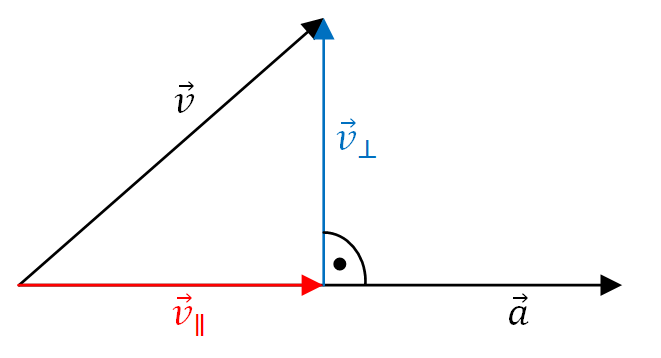
\includegraphics[width=6cm]{pics/1_Projektion.png}
				\end{minipage}
				\begin{minipage}[c]{8cm}
					\begin{equation*} P\vec{a}(\vec{v}) = |\vec{v}|\cdot \cos\alpha = \frac{\vec{a}\bullet \vec{v}}{|\vec{a}|}\end{equation*}
					\begin{equation*} v_{\parallel} = \frac{\vec{a}\bullet \vec{v}}{\vec{a}\cdot \vec{a}}\cdot \vec{a}\end{equation*}
					\begin{equation*} v_{\perp} = \vec{v} - \frac{\vec{a}\bullet \vec{v}}{\vec{a}\cdot \vec{a}}\cdot \vec{a}\end{equation*}
				\end{minipage}
		\end{enumerate}

	\subsubsection{Normalengleichung}
		\begin{equation*}
			\vec{n} \cdot (\vec{a} - \vec{p}) = 0
		\end{equation*}
		Der Normalenvektor $\vec{n}$ steht senkrecht zur Geraden oder zur Ebene. Mit seiner Hilfe und einem Punkt P ($\vec{0P} = \vec{p}$) lässt sich
		die Koordinatengleichung direkt hinschreiben:
		\begin{equation*}
			n_1x + n_2y + n_3z = \vec{n_0} \cdot \vec{p}
		\end{equation*}
		Umgekehrt lässt sich aus der Koordinatengleichung die Normalengleichung herauslesen. \\

		\textbf{Beispiel 1:} Gegebene Punkte: $A=\vektor{2}{2}{-2}$
									 $B=\vektor{3}{-3}{-1})$ \\ \ \\
							 Normale kann mithilfe des Skalarprodukts gefunden werden: \\ \ \\
									 $\vektor{n_1}{n_2}{n_3}\bullet\vektor{2}{2}{-2}=2n_1+2n_2-2n_3$ und
									 $\vektor{n_1}{n_2}{n_3}\bullet\vektor{3}{-3}{-1}=3n_1-3n_2-n_3$\\ \ \\ \ \\
							$\begin{array}{|rrr|r|}
								\hline 
									2 & 2 & -2 & 0 \\
									3 & -3 & -1 & 0 \\
								\hline
							\end{array}$
							$\rightarrow^{...}\rightarrow$	
							$\begin{array}{|rrr|r|}
								\hline 
									1 & 0 & \frac{-2}{3} & 0 \\
									0 & 1 & \frac{-1}{3} & 0 \\
								\hline
							\end{array}$
							$\rightarrow$
							$\vec{n}=\vektor{2}{1}{3}$ für $n_3 = 3$ ($n_3$ ist frei wählbar)\\
	 \textbf{Beispiel 2:} $3x-2y-z=-4\rightarrow\vec{n}=\vektor{3}{-2}{-1}$
		
\subsection{Verhalten zweier Objekte}
	\subsubsection{Schnittwinkel}
		Es wird der spitze Winkel zwischen \ldots{ }berechnet (g, h sind Geraden; E, F Ebenen; m und n Normalen):\\
		\begin{tabular}{llll}
		g $\wedge$ h:
		&$g: \vec{x}=\vec{p}+r\vec{v}$ 
		&$h: \vec{x}=\vec{q}+s\vec{w}$ 
		&$\alpha=\arccos{\frac{|v\bullet w|}{|\vec{v}|\cdot|\vec{w}|}}$\\
		g $\wedge$ h:
		&$g: m_1x+m_2y=b$
		&$h: n_1x+n_2y=c$
		&$\alpha=\arccos{\frac{|m\bullet n|}{|\vec{m}|\cdot|\vec{n}|}}$\\
		g $\wedge$ E:
		&$g: \vec{x}=\vec{p}+r\vec{v}$
		&$E: n_1x+n_2y+n_3z=b$
		&$\alpha=\arcsin{\frac{|v\bullet n|}{|\vec{v}|\cdot|\vec{n}|}}$\\
		E $\wedge$ F:
		&$E: m_1x+m_2y+m_3z=b$
		&$F: n_1x+n_2y+n_3z=c$
		&$\alpha=\arccos{\frac{|m\bullet n|}{|\vec{m}|\cdot|\vec{n}|}}$\\
		\end{tabular}

	\subsubsection{Gegenseitige Lage}
		Es werden jeweils zwei Objekte gleichgesetzt (g, h sind Geraden; E, F
		Ebenen).\\
		\begin{tabular}{lllll}
			&&$g = h$ &$g = E$ &$E = F$\\
			Keine Lösung &$\Rightarrow$ &kollinear oder windschief &parallel
			&parallel\\
			1 Lösung &$\Rightarrow$ &1 Schnittpunkt &1 Schnittpunkt & - \\
			$\infty$ Lösungen (1 Parameter frei wählbar) &$\Rightarrow$ 
			&g und h sind identisch &g liegt in E &1 Schnittgerade ($\vec{n}_E \times \vec{n}_F$) \\
			$\infty$ Lösungen (2 Parameter frei wählbar) &$\Rightarrow$  
			& - & - &E und F sind identisch
		\end{tabular}
		
	\subsubsection{Lage von Geraden}
		Es wird das Vektorprodukt von zwei Geraden gebildet (g und h sind Geraden). \\
		Wenn $\vec{g}\times\vec{h}=0$ dann sind die Geraden parallel, ansonsten sind sie windschief.

\subsection{Orthonormalisierung}
	$\vec{a_1}, \vec{a_2}, \vec{a_3}$ sind linear unabhängig $\longrightarrow \vec{b_1} \bot \vec{b_2} \bot \vec{b_3}$\\
	\begin{minipage}{3cm}
		\begin{equation*}
			\vec{b_1} = \frac{\vec{a_1}}{|\vec{a_1}|}
		\end{equation*}
	\end{minipage}
	\begin{minipage}{5cm}
		\begin{equation*}
			\vec{b_2} = \frac{\vec{a_2} - (\vec{a_2} \bullet \vec{b_1}) \vec{b_1}}{|\vec{a_2} - (\vec{a_2} \bullet \vec{b_1}) \vec{b_1}|}
		\end{equation*}
	\end{minipage}
	\begin{minipage}{5cm}
		\begin{equation*}
			\vec{b_3} = \frac{\vec{a_3} - (\vec{a_3} \bullet \vec{b_1})\vec{b_1} - (\vec{a_3} \bullet \vec{b_2})\vec{b_2}}
					{|\vec{a_3} - (\vec{a_3} \bullet \vec{b_1})\vec{b_1} - (\vec{a_3} \bullet \vec{b_2})\vec{b_2}|}
		\end{equation*}
	\end{minipage} \\ \ \\
	
	\textbf{Beispiel:} $\vec{a_1}=\vektor{1}{0}{0}
						\vec{a_2}=\vektor{1}{1}{0}
						\vec{a_3}=\vektor{1}{1}{1}$ \\
						
						$\vec{b_1}=\frac{\vektor{1}{0}{0}}{\left|\vektor{1}{0}{0}\right|}=\vektor{1}{0}{0}$ \\
						$\vec{b_2}=\frac{\vektor{1}{1}{0}-\left(\vektor{1}{1}{0}\bullet\vektor{1}{0}{0}\right)\vektor{1}{0}{0}}{\left|\vektor{1}{1}{0}-\left(\vektor{1}{1}{0}\bullet\vektor{1}{0}{0}\right)\vektor{1}{0}{0}\right|}=\vektor{1}{1}{0}$\\
						$\vec{b_3}=\frac{\vektor{1}{1}{1}-\left(\vektor{1}{1}{1}\bullet\vektor{1}{0}{0}\right)\vektor{1}{0}{0}-\left(\vektor{1}{1}{1}\bullet\vektor{1}{1}{0}\right)\vektor{1}{1}{0}}{\left|\vektor{1}{1}{1}-\left(\vektor{1}{1}{1}\bullet\vektor{1}{0}{0}\right)\vektor{1}{0}{0}-\left(\vektor{1}{1}{1}\bullet\vektor{1}{1}{0}\right)\vektor{1}{1}{0}\right|}=\vektor{0}{0}{1}$

\subsection{Mittelsenkrechte}
	\begin{equation*}
		\vec{M_{AB}} = \frac{\vec{a} + \vec{b}}{2}
	\end{equation*}

\subsection{Least Squares}
	$A^tAv = A^tb \longrightarrow$ nach $v$ auflösen und um den kleinsten Abstand zu bekommen. \qquad $(Av = b)$ \\
	$v = (A^{t} A)^{-1} A^{t} b$
		
\subsection{Vektorprodukt/Kreuzprodukt}
	\begin{equation*}
		\vec{c} = \vec{a} \times \vec{b} = \vektor{a_1}{a_2}{a_3} \times \vektor{b_1}{b_2}{b_3} = \left(\begin{array}{c}
			a_2b_3 - a_3b_2\\
			a_3b_1 - a_1b_3\\
			a_1b_2 - a_2b_1
		\end{array}\right)
		=\left(\begin{array}{c}
			\left|\begin{array}{cc}
				a_2 & b_2 \\
				a_3 & b_3 \end{array}\right|\\
			-\left|\begin{array}{cc}
				a_1 & b_1 \\
				a_3 & b_3 \end{array}\right|\\
			\left|\begin{array}{cc}
				a_1 & b_1 \\
				a_2 & b_2 \end{array}\right|
		\end{array}\right)
	\end{equation*}

	\begin{tabular}{ll}
		Zwischenwinkel: &
		\begin{equation*}
			\sin\alpha = \frac{|\vec{a} \times \vec{b}|}{|\vec{a}||\vec{b}|}
		\end{equation*}
	\end{tabular}\\ \\

	Mit Hilfe des Vektorproduktes lässt sich der \textbf{Normalenvektor}
	zweier Vektoren bestimmen. Ausserdem entspricht der Betrag des Vektorproduktes
	dem \textbf{Flächeninhalt} des von den Vektoren $\vec{a}$ und $\vec{b}$
	aufgespannten Parallelogramms. Somit sind $\vec{a}$ und $\vec{b}$ also
	kollinear, wenn $\vec{a}\times\vec{b}=0$. Das Vektorprodukt ist ein
	\textbf{Rechtssystem}
	($\vec{a} \Leftrightarrow$ Daumen; $\vec{b} \Leftrightarrow$ Zeigefinger;
	$\vec{c} \Leftrightarrow$ Mittelfinger). Das Vektorprodukt gilt nur in 3D (im
	Falle eines 2 dimensionalen Systems gilt einfach $a_3 = b_3 = 0$).

	\subsubsection{Algebraische Eigenschaften des Vektorproduktes}
		\begin{tabular}{ll}
			$\vec{a}\times\vec{b} = -(\vec{b}\times\vec{a}) = -\vec{b}\times\vec{a}$
			&(Anti-Kommutativgesetz)\\
			$(r\cdot\vec{a})\times\vec{b} = r(\vec{a}\times\vec{b}) = \vec{a}\times(r\cdot\vec{b})$
			&(gemischtes Assoziationsgesetz)\\
			$(\vec{a}+\vec{b})\times\vec{c} = (\vec{a}\times\vec{c})+(\vec{b}\times\vec{c})
			= \vec{a}\times\vec{c}+\vec{b}\times\vec{c}$\\
			$\vec{a}\times(\vec{b}+\vec{c}) = (\vec{a}\times\vec{b})+(\vec{a}\times\vec{c})
			= \vec{a}\times\vec{b}+\vec{a}\times\vec{c}$ &(Distributivgesetz)
		\end{tabular}
	
	\subsubsection{Volumen eines Parallelpipeds}
		\begin{equation*}
			det(A) = |\vec{a}; \vec{b}; \vec{c}| = (\vec{a} \times \vec{b}) \bullet \vec{c} = a_1b_2c_3 + a_2b_3c_1 + a_3b_1c_2 - c_1b_2a_3 - c_2b_3a_1 - c_3b_1a_2
		\end{equation*}

		$|\vec{a}; \vec{b}; \vec{c}| = 0 \Leftrightarrow \vec{a}; \vec{b}; \vec{c}$ komplanar \qquad 
		$|\vec{a}; \vec{b}; \vec{c}| > 0 \Leftrightarrow \vec{a}; \vec{b}; \vec{c}$ bilden Rechtssystem \qquad
		$|\vec{a}; \vec{b}; \vec{c}| < 0 \Leftrightarrow \vec{a}; \vec{b}; \vec{c}$ bilden Linkssystem

	\subsubsection{Flächeninhalt eines Dreiecks}
		$A=\frac{1}{2}|\vec{AB}\times\vec{AC}|$ \ \ wobei $\vec{AB}$ und $\vec{AC}$ Richtungsvektoren sind.
	\subsection{Flächeninhalt Polygon}
	\begin{equation*}
		A = \frac{1}{2} \left|
		\begin{array}{ccc}
			x_1 & & y_1\\
			& $X$ &\\
			x_2 & & y_2\\
			& $X$ &\\
			x_3 & & y_3\\
			& $X$ &\\
			x_n & & y_n\\
			& $X$ &\\
			x_1 & & y_1\\
		\end{array}
		\right|
		\quad \rightarrow \quad
		A = \frac{1}{2}(
		x_1 \cdot y_2 - x_2 \cdot y_1 + 
		x_2 \cdot y_3 - x_3 \cdot y_2 + ... +
		x_{n-1} \cdot y_n - x_n \cdot y_{n-1} +
		x_n \cdot y_1 - x_1 \cdot y_n) 
	\end{equation*}
	\subsubsection{Anwendung}
		Abstand Punkt/Ebene, Gerade/Gerade (windschief):
		\begin{equation*}
			d = (\vec{p_1} - \vec{p_2}) \bullet \vec{n_0} = (\vec{p_1} - \vec{p_2}) \bullet \frac{\vec{r_1} \times \vec{r_2}}{|\vec{r_1} \times \vec{r_2}|}
		\end{equation*} 

		Abstand Punkt/Gerade oder Gerade/Gerade (parallel):
		\begin{equation*}
			d = \frac{|\vec{r} \times (\vec{p} - \vec{p_0})|}{|\vec{r}|}
		\end{equation*}
%%%%%%%%%%%%%%%%%%%%%%%%%%%%%%%%%%%%%%%%%%%%%%%%
% Vektorräume
%%%%%%%%%%%%%%%%%%%%%%%%%%%%%%%%%%%%%%%%%%%%%%%%
\newpage
\section{Vektorräume}

\subsection{Rechenregeln und Definition}
	\begin{tabular}{| l | l |}
		\hline v0: & $a + b = b + a$\\
			& $a + (b + c) = (a + b) + c$\\
		\hline v1: & $0 \in \mathbb{R}, 0 = (0, \ldots, 0) \qquad v + 0 = v \qquad \forall v$\\
		\hline v2: & zu $v \in \mathbb{R}^n$ gibt es ein $-v = (-v_1, \ldots, -v_n)$ \qquad mit $v + (-v) = 0$\\
		\hline v3: & $0 \cdot v = 0 \qquad 1 \cdot v = v$\\
		\hline v4: & $\lambda(u + v) = \lambda u + \lambda v$\\
			& $(\lambda + \mu) \cdot u = \lambda u + \mu u$\\
			& $(\lambda\mu)u = \lambda(\mu u)$\\
		\hline
	\end{tabular}\\ \\

	\textbf{Def.:} Eine Menge $V$ mit den Rechenregeln v0-v4 heisst Vektorraum, $v \in V$ heissen Vektoren.

\subsection{lineare Approximation}
	\begin{equation*}
		\left(\begin{array}{c}
			a_0 + a_1x_0 + a_2{x_0}^2 + \ldots + a_n{x_0}^n\\
			a_0 + a_1x_1 + a_2{x_1}^2 + \ldots + a_n{x_1}^n\\
			\vdots \\
			a_0 + a_1x_n + a_2{x_n}^2 + \ldots + a_n{x_n}^n\\
		\end{array}\right) = \left(\begin{array}{c}
			f(x_0)\\
			f(x_1)\\
			\vdots\\
			f(x_n)
		\end{array}\right) \Rightarrow \left(\begin{array}{ccccc}
			1 & x_0 & {x_0}^2 & \ldots & {x_0}^n\\
			1 & x_1 & {x_1}^2 & \ldots & {x_1}^n\\
			\vdots & \vdots & & \vdots \\
			1 & x_n & {x_n}^2 & \ldots & {x_n}^n\\
		\end{array}\right) \cdot \left(\begin{array}{c}
			a_0\\
			a_1\\
			\vdots \\
			a_n
		\end{array}\right) = \left(\begin{array}{c}
			f(x_0)\\
			f(x_1)\\
			\vdots \\
			f(x_n)
		\end{array}\right)
	\end{equation*}

\subsection{Spur}
	Die Spur ist die Summe der Diagonalelemente einer Matrix $Spur(A) = \Sigma a_{ii}$\\
	$Spur(ABC) = Spur(CAB) = Spur(BCA) \rightarrow$ zyklisch vertauschbar


\subsection{Basis}
	\textbf{Def.:} Sei also $V$ ein Vektorraum. Eine Menge $B = \lbrace b_1, b_2, \ldots \rbrace$ linear unabhängiger Vektoren
	ist eine Basis, wenn jeder Vektor von $V$ als Linearkombination von Vektoren aus $B$ dargestellt werden kann. Ein 
	Vektorraum heisst endlichdimensional, wenn er eine endliche Basis hat. 

\subsection{Basistransformation}
	\begin{minipage}{7cm}
		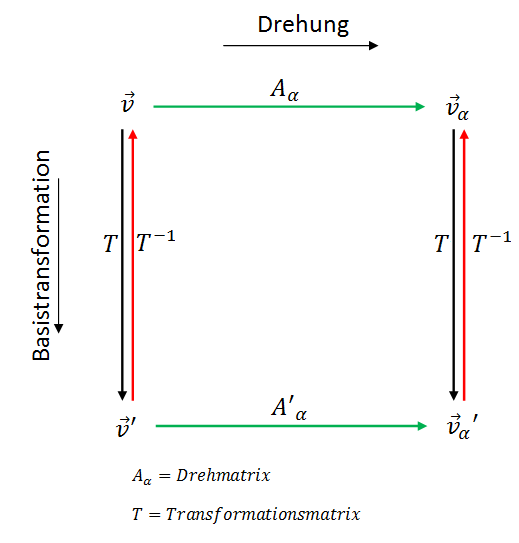
\includegraphics[width=7cm]{pics/2_Basistransformation.png}
	\end{minipage}
	\begin{minipage}{7cm}
		\begin{tabular}{ll}
			& $A =$ Matrix in alter Basis\\
			$A' = TAT^{-1}$ & $A' =$ Matrix in neuer Basis\\
			& $T =$ Transformationsmatrix\\
			$\xi' = T\xi$& $\xi =$ Vektor in der alten Basis\\
			& $\xi' =$ Vektor in der neuen Basis
		\end{tabular}
	\end{minipage}

	\subsubsection{Bestimmen der Transformationsmatrix $T$}
		$B = \underbrace{\lbrace b_j \rbrace}_{alte Basis} \qquad B' = \underbrace{\lbrace b_j' \rbrace}_{neue Basis}$\\ \\

		\textbf{Variante 1 (mit $\beta$):}\\
		Mit Gleichungssystem herausfinden, wie viele von der neuen Basis gebraucht wird um die alte darzustellen.\\
		$b_j = \beta_{j1}b_1' + \beta_{j2}b_2' + \ldots + \beta_{jn}b_n' \rightarrow$ daraus folgt $\beta$\\
		\begin{equation*}
			\mathbf{T = \beta^t}
		\end{equation*}

		\textbf{Variante 2:}\\
		Oftmals ist $b_j'$ mit den Koordinaten von der alten Basis angegeben\\
		$b_j' = \beta_{j1}b_1 + \beta_{j2}b_2 + \ldots + \beta_{jn}b_n$\\
		$\Rightarrow$ Koordinaten in der alten Basis von $b_j'$ in die Spalten der Matrix einfüllen, welches gleich $\mathbf{T^{-1}}$ ist.\\
		\begin{equation*}
			\mathbf{T = (T^{-1})^{-1}}
		\end{equation*}

	\subsubsection{Eigenschaften einer Basistransformation}
		Ein Basiswechsel ändert die Spur und die Determinante nicht!\\
		\begin{equation*}
			Spur(TAT^{-1}) = Spur(T^{-1}TA) = Spur(A)
		\end{equation*}
		\begin{equation*}
			det(TAT^{-1}) = det(T^{-1}) \cdot det(A) \cdot det(T) = det(A)
		\end{equation*}

\subsection{Lineare Abbildungen}
	$ T \cdot \vec{v} = \vec{v'} $
	oder $ T \cdot A = A'  \rightarrow T = A' \cdot A^{-1} $
	\subsubsection{Orientierung}
		\begin{tabular}{lp{13cm}}
			$GL_n(\mathbb{R}) = \lbrace A | det(A) \neq 0\rbrace$ & "general linear group'' enthält alle lineare Abbildungen\\
			& $det(A)\left\lbrace\begin{array}{cc}
				>0 & \text{Rechtssystem}\\
				<0 & \text{Linkssystem}
				\end{array}\right.$ \\ \\

			$SL_n(\mathbb{R}) = \lbrace A | det(A) = 1 \rbrace$ &  ''special linear group'' enthält alle volumen- und orientierungstreue Matrizen\\
			& $det(A) =$ Volumenänderungsfaktor \\ \\

			$O(n) = \lbrace A | A^tA = E \rbrace$ & enthält alle orthogonalen Matrizen, die Längen und Winkel bleiben erhalten.\\
			& Die Detereminante ist dabei $det(A) = \pm1$ (Zeilen-/Spaltenvektoren sind orthogonal) ($OO^t = E$)
		\end{tabular}\\ \\

		\begin{tabular}{ll}
			$SO(n) = \lbrace A \in GL_n(\mathbb{R}) | det(A) = 1, A^tA = E \rbrace$ & Drehmatrizen, Volumen, Längen und Winkel bleiben 					erhalten.
		\end{tabular}

	\subsubsection{Drehwinkel}
		\begin{tabular}{p{5cm}l}
			in $SO(2)$ & \begin{equation*}
				\cos\alpha = \frac{Spur(D_\alpha)}{2}
			\end{equation*} \\ \\
			
			in $SO(3)$ ohne Spiegelung & \begin{equation*}
				\cos\alpha = \frac{Spur(D_\alpha) - 1}{2}
			\end{equation*}\\ \\

			 in $SO(3)$ mit Spiegelung & \begin{equation*}
				\cos\alpha = \frac{Spur(D_\alpha) + 1}{2}
			\end{equation*}
		\end{tabular}
		
	\subsubsection{einige Lineare Abbildungen}
		\begin{tabular}{llll}
			$A=	\left(\begin{array}{ll}0 &1 \\1 &0\end{array}\right)$ 
        			&$\Rightarrow$ Spiegelung an Geraden $x_2=x_1$
			&$A=	\left(\begin{array}{ll}0 &-1 \\1 &0\end{array}\right)$ 
            		&$\Rightarrow$ Drehung um $\vec{O}$ mit $+90^{\circ}$\\
			$A=	\left(\begin{array}{ll}1 &1 \\0 &1\end{array}\right)$ 
            		&$\Rightarrow$ Scherung $\|$ zur $x_1$-Achse um $45^{\circ}$
			&$A=	\left(\begin{array}{ll}\cos{\alpha} &-\sin{\alpha} \\\sin{\alpha} &\cos{\alpha}\end{array}\right)$ 
            		&$\Rightarrow$ Drehung um $\vec{O}$ mit $\alpha$\\			
			$A=	\left(\begin{array}{llc}1 &0 &0 \\0 &1 &0 \\0 &0 &-1\end{array}\right)$ 
            		&$\Rightarrow$ Spiegelung  $x_1x_2$ -Ebene
			&$A=	\left(\begin{array}{lll}-1 &0 &0 \\0 &-1 &0 \\0 &0 &-1\end{array}\right)$ 
            		&$\Rightarrow$ Punktspiegelung an $\vec{O}$\\	
			$A=	\left(\begin{array}{lll}2 &0 &0 \\0 &2 &0 \\0 &0 &2\end{array}\right) $
			&$\Rightarrow\begin{array}{l}\mbox{Streckung von } \vec{O} \mbox{ aus} \\ \mbox{mit Faktor 2} \end{array}$
			&$A=	\left(\begin{array}{lll}\cos{\alpha} &-\sin{\alpha} &0 \\ \sin{\alpha}
			&\cos{\alpha} &0 \\0 &0 &1\end{array}\right)$ 
			&$\Rightarrow \begin{array}{l}\mbox{Drehung des Raumes}\\ \mbox{um die } x_3
			\mbox{-Achse mit } \alpha \end{array}$										
		\end{tabular}

	\subsubsection{Projektionsmatrix bzw. Kameraprojektionsmatrix}
		Eine Kameraprojektionsmatrix beschreibt die Abbildung eines Bildpunkt von einem 3D-Objekt auf eine Kamera.		
		\begin{itemize}
			\item Eine Kameraprojektionsmatrix hat diese Form.
				\begin{equation*}
				P = KD (E - \vec{c})
				\qquad
				(E-\vec{c})=\left(\begin{array}{cccc}
				1 & 0 & 0 &-c_x\\
				0 & 1 & 0 &-c_y\\
				0 & 0 & 1 &-c_z
				\end{array}\right)
				\qquad
					\begin{array}{rcl}
						\vec{c} & \hat{=} & $Kameraposition$\\
						D & \hat{=} & $Drehmatrix$
					\end{array}
				\end{equation*}
			\item Bildpunkte berechnen
				\begin{equation*}
					\tilde{b} = P \tilde{q}
				\end{equation*}
				Um nun $\vec{b}$ zu berechnen muss man $\tilde{b}$ mit der dritten Komponenten dividieren.
			
			\item Eine Kameraabbildungsmatrix hat diese Form.
				\begin{equation*}
					$K = $
					\begin{bmatrix}[ccc]
						f	&	0	&	\color{red} mx	\\
						0 	&	f	&	\color{red} my	\\
						0	&	0	&	1
					
					\end{bmatrix}
					$*$
					\begin{bmatrix}[c]
						qx	\\
						qy 	\\
						qz	
					
					\end{bmatrix}
					$$
					\text{ mit}
					$$
						\text{ f = Brennweite, \color{red} mx \color{black} = $\frac{1}{2}$ Anzahl Pixel auf x, \color{red} my \color{black} = $\frac{1}{2}$ Anzahl Pixel auf y}
					$$
				\end{equation*}
				
			\item Eine Gerade, die durch den Bildpunkt und durch das 3D-Objekt geht, wird in dieser Form beschrieben.
				\begin{equation*}
					\vec{p} = \vec{c} + s \vec{r}
				\end{equation*}
			
				\begin{itemize}
					\item Der Richtungsvektor $\vec{r}$ wird so berechnet $\vec{r}=(KD)^{-1} \tilde{b}$
					
				\end{itemize}
		
			\item Schnittpunkt zweier Geraden wird in dieser Form beschrieben.\\
				\begin{equation*}
				A\vec{x}=\vec{b} \rightarrow
				\underbrace{\left(\begin{array}{ccccc}
					" "&" "&" "&" "& 0\\
					" "& E &" "&-\vec{r_1}&0\\
					" "&" "&" "&" "& 0\\
					" "&" "&" "& 0 & " "\\
					" "& E &" "& 0 &-\vec{r_2}\\
					" "&" "&" "& 0 & " "
					\end{array}\right)}_{\displaystyle A}\cdot
				\underbrace{\left(\begin{array}{c}
					x\\y\\z\\t\\s
					\end{array}\right)}_{\displaystyle\vec{x}} = 
				\underbrace{\left(\begin{array}{c}
					" "\\\vec{c_1}\\" "\\" "\\\vec{c_2}\\" "
					\end{array}\right)}_{\displaystyle\vec{b}}\\
				\end{equation*}\\
				Da dieses System überbestimmt ist gibt es im Normalfall keine Lösung (Geraden Schneiden sich nicht). Um aber trotzdem einen Punkt zu finden muss man das Least-Square Verfahren durchführen.\\[0.2cm]
				$A^t \cdot A \cdot \vec{x} = A^t \cdot \vec{b}
				\quad \rightarrow \quad
				\vec{x} = (A^t \cdot A)^{-1} \cdot A^t \cdot \vec{b}$
		\end{itemize}
			

	\subsubsection{Algebraische Eigenschaften von linearen Abbildungen}
		\begin{minipage}{10cm}
			\begin{tabular}{ll}
				$A \cdot B \neq B \cdot A$ & (Anti-Kommunitativgesetz)\\
				$(A \cdot B)C = A(B \cdot C) = A \cdot B \cdot C$ & (Assoziativgesetz)
			\end{tabular}\\ \\
			\textbf{Verkettung von lin. Abbildungen}\\
			\textbf{$\rightarrow$ Zeile mal Spalte}\\
				$$C=B\circ A=B(A(\vec{x}))$$
		\end{minipage}
		\begin{minipage}{7cm}
			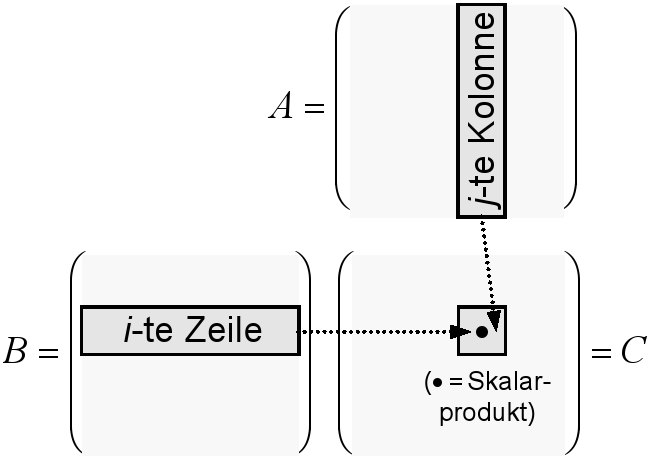
\includegraphics[width=5cm]{pics/3_Matrizenmulti}
		\end{minipage}

\subsection{Allgemeines Skalarprodukt}
	\begin{tabular}{ll}
		$\xi \bullet  \gamma = \xi^tG\gamma$ & $\xi, \gamma$ sind Vektoren\\
		$\xi' \bullet \gamma' = {\xi'}^tG'\gamma' = \xi^tT^tG'T\gamma$ & G = Symmetrische Matrix\\
		$G = T^tG'T$ & G in Standartbasis = Einheitsmatrix (E)\\
		$G' = {T^{-1}}^tGT^{-1}$ &
	\end{tabular}























%%%%%%%%%%%%%%%%%%%%%%%%%%%%%%%%%%%%%%%%%%%%%%%%
% Zerlegungen
%%%%%%%%%%%%%%%%%%%%%%%%%%%%%%%%%%%%%%%%%%%%%%%%

\section{Zerlegungen}

\subsection{L-U-Zerlegung} \label{L-U-Zerlegung}
	A = LU\\
	(A gegeben)
	\begin{enumerate}
		\item Gauss (Vorwärtsreduktion)
		\item L $\rightarrow$ Pivospalten (rot und blau), U $\rightarrow$ "Rest" (grün) 
	\end{enumerate}\ 
	$\begin{array}{|cccc|}
		\hline 
		\color{red}* & * & * & *\\
		\color{blue}* & * & * & *\\
		\color{blue}* & * & * & *\\
		\color{blue}* & * & * & *\\
		\hline
	\end{array}$
	$\rightarrow$
	$\begin{array}{|cccc|}
		\hline 
		1 & * & * & *\\
		0 & \color{red}* & * & *\\
		0 & \color{blue}* & * & *\\
		0 & \color{blue}* & * & *\\
		\hline
	\end{array}$
	$\rightarrow^{...}\rightarrow$
	$\begin{array}{|cccc|}
		\hline 
		1 & * & * & *\\
		0 & 1 & * & *\\
		0 & 0 & 1 & *\\
		0 & 0 & 0 & \color{red}*\\
		\hline
	\end{array}$
	$\rightarrow$
	$\begin{array}{|cccc|}
		\hline 
		\color{green}1 & \color{green}* & \color{green}* & \color{green}*\\
		0 & \color{green}1 & \color{green}* & \color{green}*\\
		0 & 0 & \color{green}1 & \color{green}*\\
		0 & 0 & 0 & \color{green}1\\
		\hline
	\end{array}$\ \ \ \
	$L=	\left(\begin{array}{cccc}
			\color{red}* & 0 & 0 & 0\\
		 	\color{blue}* & \color{red}* & 0 & 0\\
			\color{blue}* & \color{blue}* & \color{red}* & 0\\
			\color{blue}* & \color{blue}* & \color{blue}* & \color{red}*\\
	\end{array}\right)$\ \ \ \ \ \ 
	$U=	\left(\begin{array}{cccc}
			\color{green}* & \color{green}* & \color{green}* & \color{green}*\\
		 	0 & \color{green}* & \color{green}* & \color{green}*\\
			0 & 0 & \color{green}* & \color{green}*\\
			0 & 0 & 0 & \color{green}*\\
	\end{array}\right)$\\\\\\\\
	\textbf{Beispiel:}\ \ \ \  
	$A=	\left(\begin{array}{ccc}
		-1 &\ \ 0 &\ \ 2\\
		 \ \ 1 &\ \ 3 &\ \ 3\\
		-1 &-3 &\ \ 1\\
	\end{array}\right)$\\\\\\ 
	$\begin{array}{|ccc|}
			\hline 
			\color{red}-1 & \ \ 0 & \ \ 2\\
			\color{blue}\ \ 1 & \ \ 3 & \ \ 3\\
			\color{blue}-1 & -3 & \ \ 1\\
			\hline
	\end{array}$
	$\rightarrow$
	$\begin{array}{|ccc|}
			\hline 
			\ \ 1 & \ \ 0 & -2\\
			\ \ 0 & \color{red}\ \ 3 & \ \ 5\\
			\ \ 0 & \color{blue}-3 & -1\\
			\hline
	\end{array}$
	$\rightarrow$
	$\begin{array}{|ccc|}
			\hline 
			\ \ 1 & \ \ 0 & -2\\
			\ \ 0 & \ \ 1 & \ \ \frac 5 3\\
			\ \ 0 & \ \ 0 & \color{red}\ \ 4\\
			\hline
	\end{array}$
	$\rightarrow$
	$\begin{array}{|ccc|}
			\hline 
			\color{green}\ \ 1 & \color{green}\ \ 0 & \color{green}-2\\
			\ \ 0 & \color{green}\ \ 1 & \color{green}\ \ \frac 5 3\\
			\ \ 0 & \ \ 0 & \color{green}\ \ 1\\
			\hline
	\end{array}$\ \ \ \ \	
	$L=	\left(\begin{array}{ccc}
			\color{red}-1 &\ \ 0 &\ \ 0\\
		 	\color{blue}\ \ 1 &\color{red}\ \ 3 &\ \ 0\\
			\color{blue}-1 &\color{blue} -3 &\color{red}\ \ 4\\
	\end{array}\right)$\ \ \ \ \ \ 
	$U=	\left(\begin{array}{ccc}
			\color{green}\ \ 1 &\color{green}\ \ 0 &\color{green}-2\\
		 	\ \ 0 &\color{green}\ \ 1 &\color{green}\ \ \frac 5 3\\
			\ \ 0 &\ \ 0 &\color{green}\ \ 1\\
	\end{array}\right)$\\
		
\subsection{L-R-Zerlegung}
\begin{enumerate}
	\item L-U-Zerlegung machen gemäss \ref{L-U-Zerlegung}
	\item Matrix D berechnen (Diagonalelemente von L)\\
		$D=\left(\begin{array}{ccc}
			l_{11} & 0 & 0\\
			0 & l_{22} & 0\\
			0 & 0 & l_{33}
		\end{array}  \right)$
	\item L' und R berechnen\\
		$L'=LD^{-1}$\\
		$R=DU$\\
		\textbf{Beispiel} gem. \ref{L-U-Zerlegung}: \quad
		\begin{equation*}
			L=\left(\begin{array}{ccc}
			\color{red}-1 & 0 & 0\\
			\color{blue} 1 &\color{red} 3 & 0\\
			\color{blue}-1 &\color{blue} -3 &\color{red} 4\\
			\end{array}\right)
			\quad U=\left(\begin{array}{ccc}
			\color{green} 1 &\color{green} 0 &\color{green}-2\\
			0 &\color{green} 1 &\color{green} \frac 5 3\\
			0 & 0 &\color{green} 1\\
			\end{array}\right) \quad
			D=\left(\begin{array}{ccc}
			\color{red}-1 & 0 & 0\\
			 0 &\color{red} 3 & 0\\
			0 & 0 &\color{red} 4\\
			\end{array}\right)
		\end{equation*}
		\begin{equation*}
			L'=LD^{-1}=\left(\begin{array}{ccc}
			-1 & 0 & 0\\
			 1 & 3 & 0\\
			-1 & -3 & 4\\
			\end{array}\right)
			\left(\begin{array}{ccc}
			-1 & 0 & 0\\
			0 & \frac 1 3 & 0\\
			0 & 0 & \frac 1 4\\
			\end{array}\right)
			= \left(\begin{array}{ccc}
			1 & 0 & 0\\
			-1 & 1 & 0\\
			1 & -1 & 1\\
			\end{array}\right)
		\end{equation*}
		
		\begin{equation*}
			R=DU=\left(\begin{array}{ccc}
			-1 & 0 & 0\\
			0 & 3 & 0\\
			0 & 0 & 4\\
			\end{array}\right)
			\left(\begin{array}{ccc}
			1 & 0 & -2\\
			0 & 1 & \frac 5 3\\
			0 & 0 & 1\\
			\end{array}\right)
			=\left(\begin{array}{ccc}
			-1 & 0 & 2\\
			0 & 3 & 5\\
			0 & 0 & 4\\
			\end{array}\right)
		\end{equation*}
\end{enumerate}
\clearpage
\subsection{Q-R-Zerlegung / Gram-Schmidt-Zerlegung}
	A = QR\\
	(A gegeben)
	\begin{enumerate}
		\item Q $\rightarrow$ A orthonormalisieren 
		\item R $\rightarrow$ $Q^t$A 
	\end{enumerate} 
	\textbf{Beispiel:}\ \ \ \  
	$A=	\left(\begin{array}{ccc}
		\ \ 1 &\ \ 0 &\ \ 0\\
		\ \ 1 &\ \ 1 &\ \ 0\\
		\ \ 1 &\ \ 1 &\ \ 1\\
	\end{array}\right)$
	$\rightarrow^{orthonorm.}\rightarrow$
	$\left(\begin{array}{ccc}
		\ \ \frac 1 {\sqrt 3}  & -\frac 2 {\sqrt 6} &\ \ 0\\
		\ \ \frac 1 {\sqrt 3} &\ \ \frac 1 {\sqrt 6} & -\frac 1 {\sqrt 2}\\
		\ \ \frac 1 {\sqrt 3} &\ \ \frac 1 {\sqrt 6} &\ \ \frac 1 {\sqrt 2}\\
	\end{array}\right)$ = Q\\\\\\
	R = $Q^t$A = 
	$\left(\begin{array}{ccc}
			\ \ \frac 1 {\sqrt 3}  &\ \ \frac 1 {\sqrt 3} &\ \frac 1 {\sqrt 3}\\
			 -\frac 2 {\sqrt 6} &\ \ \frac 1 {\sqrt 6} &\ \frac 1 {\sqrt 6}\\
			\ \ 0 & -\frac 1 {\sqrt 2} &\ \ \frac 1 {\sqrt 2}\\
		\end{array}\right)$ * 
	$\left(\begin{array}{ccc}
		\ \ 1 &\ \ 0 &\ \ 0\\
		\ \ 1 &\ \ 1 &\ \ 0\\
		\ \ 1 &\ \ 1 &\ \ 1\\
	\end{array}\right)$ =
	$\left(\begin{array}{ccc}
		\ \ \frac 3 {\sqrt 3} &\ \ \frac 2 {\sqrt 3} &\ \ \frac 1 {\sqrt 3}\\
		\ \ 0 &\ \ \frac 2 {\sqrt 6} &\ \ \frac 1 {\sqrt 6}\\
		\ \ 0 &\ \ 0 &\ \ \frac 1 {\sqrt 2}\\
	\end{array}\right)$

\subsection{Cholesky-Zerlegung}
	A = $LL^t$\\
	(A gegeben)\\\\ 
	$A=	\left(\begin{array}{ccc}
		\ \ l_{11} &\ \ l_{21} &\ \ l_{31}\\
		\ \ l_{12} &\ \ l_{22} &\ \ l_{32}\\
		\ \ l_{13} &\ \ l_{23} &\ \ l_{33}\\	
	\end{array}\right)$ 
	= $LL^t$ = 
	$\left(\begin{array}{ccc}
		\ \ x_1 &\ \ 0 &\ \ 0\\
		\ \ x_2 &\ \ x_4 &\ \ 0\\
		\ \ x_3 &\ \ x_5 &\ \ x_6\\	
	\end{array}\right)$ *
	$\left(\begin{array}{ccc}
		\ \ x_1 &\ \ x_2 &\ \ x_3\\
		\ \ 0 &\ \ x_4 &\ \ x_5\\
		\ \ 0 &\ \ 0 &\ \ x_6\\	
	\end{array}\right)$\\\\\\ 
	(1): $x_1*x_1 + 0*0 + 0*0 = x_1^2 = l_{11}$ $\rightarrow$ $x_1$ berechnen\\ 		
	(2): $x_2*x_1 + x_4*0 + 0*0 = x_2*x_1 = l_{12}$ $\rightarrow$ $x_2$ berechnen\\ 
	(3): $x_3*x_1 + x_5*0 + x_6*0 = x_3*x_1 = l_{13}$ $\rightarrow$ $x_3$ berechnen\\
	(4): $x_2*x_2 + x_4*x_4 + 0*0 = x_2^2 + x_4^2 = l_{22}$ $\rightarrow$ $x_4$ berechnen\\
	(5): $x_3*x_2 + x_5*x_4 + x_6*0 = x_3*x_2 + x_5*x_4 = l_{23}$ $\rightarrow$ $x_5$ berechnen\\	
	(6): $x_3*x_3 + x_5*x_5 + x_6*x_6 = x_3^2 + x_5^2 + x_6^2 = l_{33}$ $\rightarrow$ $x_6$ berechnen\\	








%%%%%%%%%%%%%%%%%%%%%%%%%%%%%%%%%%%%%%%%%%%%%%%%
% Eigenwerte und Eigenvektoren
%%%%%%%%%%%%%%%%%%%%%%%%%%%%%%%%%%%%%%%%%%%%%%%%
\section{Eigenwerte und Eigenvektoren}
	Wenn eine Abbildung auf denselben Punkt fällt ($\vec{v} = \vec{v}'$), nennt man dies Eigenfixpunkt.
	Der Eigenvektor $\vec{v}$ zeigt nun in diese Richtung (als Gerade) und der Eigenwert $\lambda$ gibt den Faktor an, mit der in
	diese Richtung gezeigt wird. D.h. es gilt
	\begin{equation*}
		Av = \lambda v
	\end{equation*}

	\textbf{Def.:} Eine Matrix heisst diagonalisierbar, wenn es eine Basis aus den Eigenvektoren gibt.\\

	\textbf{Def.:} Symmetrische Matrizen sind diagonalisierbar (die Eigenwerte stehen in der Diagonalen). 
	Es gibt eine orthonormierte Eigenvektorbasis.

	\subsection{Berechnen der Eigenwerte}
		\begin{enumerate}
			\item Determintante ausrechnen
			\item Gleichung lösen (Lösungen = Eigenwerte)
		\end{enumerate}
		\begin{equation*}
			det(A - \lambda E) = 0
		\end{equation*}
		
		Beispiel:
		\begin{equation*}
			A = \left(\begin{array}{cc}
				a_1 & b_1\\
				a_2 & b_2
			\end{array}\right) \\ \Longrightarrow\\
			\left|\begin{array}{cc}
				a_1 - \lambda & b_1\\
				a_2 & b_2 - \lambda
			\end{array}\right| = 0 \\ \Longrightarrow\\
			\lambda^2 -\lambda(a_1 + b_2) + a_1b_2 - a_2b_1 = 0
		\end{equation*}
		
		\textbf{Def.:} $det(A - \lambda E)$ heisst charakteristisches Polynom $\chi_A$\\

	\subsection{Berechnen der Eigenvektoren}
		\textbf{Für jeden Eigenwert $\lambda_i$}  Gleichungssystem aufstellen und mit Gauss auflösen $\Rightarrow$ eine Zeile
		verschwindet $\Rightarrow \infty$ Lösungen $\Rightarrow$ Wert von verschwundener Zeile frei wählbar.
		\begin{equation*}
			(A - \lambda_i E)\vec{v_i} = 0
		\end{equation*}

		Beispiel:
		\begin{equation*}
			\left|\begin{array}{ccc}
				v_1 - 2v_2 & = & 0\\
				0 & = & 0
			\end{array}\right| \\
			\Rightarrow \\
			v_2 \text{ ist frei wählbar} \\
			\Rightarrow \\
			\begin{array}{c}
				v_1 = 2v_2\\
				v_2 = x
			\end{array} \\
			\Rightarrow \\
			\vec{v} = \left(\begin{array}{c}
				v_1 \\
				v_2
			\end{array}\right) = \left(\begin{array}{c}
				2v_2\\
				v_2
			\end{array}\right) = \left(\begin{array}{c}
				2x \\
				x
			\end{array}\right) = x \cdot \left(\begin{array}{c}
				2 \\
				1
			\end{array}\right)
		\end{equation*}\\
	Eigenvektoren von symmetrischen Matrizen sind immer senkrecht zueinander.\\
	
		\begin{minipage}{0.5\textwidth}
			\subsection{Potenzrechen von Matrizen}
			\begin{equation*}
				A^k = T^{-1}{A'}^kT = T^{-1}\left(\begin{array}{ccc}
					{\lambda_1}^k & & 0\\
					& \ddots & \\
					0 & & {\lambda_n}^k
				\end{array}\right) T
			\end{equation*}
			\begin{equation*}
				A' = \left(\begin{array}{ccc}
					{\lambda_1}^k & & 0\\
					& \ddots & \\
					0 & & {\lambda_n}^k
				\end{array}\right) 
				A' \text{ in Eigenvektoren-Basis}
			\end{equation*}
			\begin{equation*}
				T = (Ev_1, Ev_2, \ldots, Ev_n)^{-1}
			\end{equation*}
		\end{minipage}
		\begin{minipage}{0.5\textwidth}
			\subsubsection{Eingenschaften von A'}
			\begin{itemize}
				\item $det(A') = det(A)$
				\item $det(A') = \prod_{i=1}^{n} \lambda_i$
				\item $det(T \cdot A \cdot T^{-1}) = det(A) \cdot det(T) \cdot det(T^{-1}) = det(A)$
				\item $A'=T \cdot A \cdot T^{-1}$
			\end{itemize}
		\end{minipage}

	\subsection{Rekursionsformel}
		$x_{n+3} = 4x_n - 11x_{n+1} + 6x_{n+2}$\\
		\begin{enumerate}
			\item Matrix/Vektor Schreibweise : $\left(\begin{array}{c}
					x_{n+3}\\
					x_{n+2}\\
					x_{n+1}
				\end{array}\right) = A\left(\begin{array}{c}
					x_{n+2}\\
					x_{n+1}\\
					x_n
				\end{array}\right) \qquad \qquad A = \left(\begin{array}{ccc}
					6 & -11 & 4\\
					1 & 0 & 0\\
					0 & 1 & 0
				\end{array}\right)$

			\item $\vec{u}$ ein Eigenvektor von $A$ \qquad $A^nu = \lambda^nu$ \\
				$\left(\begin{array}{c}
					x_{n+2}\\
					x_{n+1}\\
					x_n
				\end{array}\right) = 
				a_1{\lambda_1}^n\vec{u_1}+a_2{\lambda_2}^n\vec{u_2}+ a_3{\lambda_3}^n\vec{u_3} =
				a_1{\lambda_1}^n\left(\begin{array}{c}
					u_{11}\\
					u_{12}\\
					u_{13}
				\end{array}\right) + a_2{\lambda_2}^n\left(\begin{array}{c}
					u_{21}\\
					u_{22}\\
					u_{23}
				\end{array}\right) + a_3{\lambda_3}^n\left(\begin{array}{c}
					u_{31}\\
					u_{32}\\
					u_{33}
				\end{array}\right)$ \\
				$x_n = a_1{\lambda_1}^nu_{13} + a_2{\lambda_2}^nu_{23} + a_3{\lambda_3}^nu_{33}$
		\end{enumerate}

\clearpage
\section{Rezepte}

\subsection{Potenzrechnen}
\textbf{Kurzanleitung:}
\begin{enumerate}
	\item Gleichung aufschreiben $A^k=T^{-1} \cdot {A'}^k \cdot T$
	\item Eigenbasis aus n linear unabhängigen Eigenvektoren finden.
	\item Basis-Transformationsmatrix T berechnen.
	\item Diagonalisierte Matrix A' berechnen.
	\item $A^k$ berechnen.
\end{enumerate}
\textbf{Schritt für Schritt Anleitung:}
\begin{enumerate}
	\item Gleichung aufschreiben:\\
		$A^k=T^{-1} \cdot {A'}^k \cdot T\qquad A =\left(\begin{array}{cc}
			3 & 2\\
			1 & 2
		\end{array}\right)$
	\item Basis aus Eigenvektoren finden\\
		\begin{enumerate}
			\item Eigenwerte berechnen:
				$ det(A-\lambda E) = 0 \qquad \left|\begin{array}{cc}
				3-\lambda & 2\\
				1 & 2-\lambda
				\end{array}\right| = (3-\lambda)(2-\lambda)-1 \cdot 2 = 0 $\\[0.2cm]
				$= \lambda^2-5\lambda+4 = 0 \rightarrow (\lambda-1)(\lambda-4)=0 \rightarrow \lambda_1 = 1 \rightarrow \lambda_2 = 4$
			\item Eigenvektoren finden:\\
			\begin{minipage}{0.5\textwidth}
				$(A-\lambda_1 E)\cdot \vec{v_1} = 0$\\
				$\begin{array}{|cc|c|}
					\hline
					2 & 2 & 0\\
					1 & 1 & 0\\
					\hline
				\end{array} 
				\begin{array}{l}
				\rightarrow 2x_1 + 2y_1 = 0\\\rightarrow 1x_1 + 1y_1 = 0\end{array}
				\rightarrow\vec{v_1} = \left(\begin{array}{c} -1\\1 \end{array}\right)$
			\end{minipage}
			\begin{minipage}{0.5\textwidth}
				$(A-\lambda_2 E)\cdot \vec{v_2} = 0$\\
				$\begin{array}{|cc|c|}
				\hline
				-1 & 2 & 0\\
				1 & -2 & 0\\
				\hline
				\end{array} 
				\begin{array}{l}
				\rightarrow -1x_2 + 2y_2 = 0\\\rightarrow 1x_2 - 2y_1 = 0\end{array}
				\vec{v_2} = \left(\begin{array}{c} 2\\1 \end{array}\right)$
			\end{minipage}
		\end{enumerate}
	\item $T$ und $T^{-1}$ berechnen:\\[0.2cm]
		\begin{minipage}
			{0.5\textwidth}$T^{-1}=(\vec{v_1} \quad \vec{v_2}) = \left(\begin{array}{cc}-1 & 2 \\ 2 & 1\end{array}\right)$
		\end{minipage}
		\begin{minipage}{0.5\textwidth}
			$T=T^{-1^{-1}}= (\vec{v_1} \quad \vec{v_2})^{-1} = \displaystyle \frac 1 3 \left(\begin{array}{cc}-1 & 2 \\ 1 & 1\end{array}\right)$
		\end{minipage}
	\item Diagonal Matrix A' berechnen:\\
		$A' = \left(\begin{array}{cc} \lambda_1 & 0\\ 0 & \lambda_2 \end{array}\right) = \left(\begin{array}{cc} 1 & 0\\ 0 & 4 \end{array}\right)$
		
	\item $A^k$ berechnen:\\
		$A^k=T^{-1} \cdot {A'}^k \cdot T = 
		\left(\begin{array}{cc}-1 & 2 \\ 2 & 1\end{array}\right) \cdot
		\left(\begin{array}{cc} 1^k & 0\\ 0 & 4^k \end{array}\right) \cdot
		\displaystyle \frac 1 3 \left(\begin{array}{cc}-1 & 2 \\ 1 & 1\end{array}\right)$
\end{enumerate}
\clearpage
\subsection{Kameraabbildungen}

\subsubsection{Bildpunkt zum 3D Punkt}
\textbf{Gegeben:}\\
\begin{tabular}{llcll}
	Brennweite: & $f=100$pixel &\quad& Bild grösse: & $m_x \cdot m_y =120 \cdot 90$\\
	Position Kameras: & $C_1=(100;0;0) \quad C_2=(0;100;0)$ && Bildpunkte: & $B_1=(36;40) \quad B_2=(65;58)$\\
	Drehmatrix $D_1$: & $D_1=\left(\begin{array}{ccc} 
	0 & -1 & 0\\
	0 & 0 & 1\\
	-1 & 0 & 0 
	\end{array}\right)  $ && Drehmatrix $D_2$: & $D_2=\left(\begin{array}{ccc} 
	0 & 0 & -1\\
	1 & 0 & 0\\
	0 & -1 & 0 
	\end{array}\right)  $
\end{tabular}\\[0.4cm]
\textbf{Gesucht:} Punkt $Q$ welche auf den Bildpunkten $B_1$ \& $B_2$ dargestellt ist.\\
\begin{enumerate}
	\item Kameramatrix aufstellen\\
		$K=\left(\begin{array}{ccc}
			f & 0 & mx/2\\
			0 & f & my/2\\
			0 & 0 & 1
		\end{array}\right) = \left(\begin{array}{ccc}
		100 & 0 & 60\\
		0 & 100 & 45\\
		0 & 0 & 1
		\end{array}\right)$
	\item Eine Gerade pro Kamera berechnen mit je einem $\vec{c_i}$ = Stützvektor und einem Richtungsvektor\\ $\vec{r_i}=(KD_i)^{-1}\cdot \vec{\tilde{b_i}} \rightarrow \vec{\tilde{b_i}} = \vektor{b_{ix}}{b_{iy}}{1}$\\
	\begin{equation*}
	\vec{r_1}=(KD_1)^{-1}\cdot \vec{\tilde{b_1}} =
	\left[\left(\begin{array}{ccc}
	100 & 0 & 60\\
	0 & 100 & 45\\
	0 & 0 & 1
	\end{array}\right)
	\left(\begin{array}{ccc}
	0 & -1 & 0\\
	0 & 0 & 1\\
	-1 & 0 & 0 
	\end{array}\right)\right]^{-1}\cdot
	\vektor{36}{60}{1}=\vektor{-1.00}{" "0.24}{-0.05}
	\end{equation*}\\
	\begin{equation*}
	\vec{r_2}=(KD_2)^{-1}\cdot \vec{\tilde{b_2}} =
	\left[\left(\begin{array}{ccc}
	100 & 0 & 60\\
	0 & 100 & 45\\
	0 & 0 & 1
	\end{array}\right)
	\left(\begin{array}{ccc}
	0 & 0 & -1\\
	1 & 0 & 0\\
	0 & -1 & 0 
	\end{array}\right)\right]^{-1}\cdot
	\vektor{65}{58}{1}=\vektor{" "0.13}{-1.00}{-0.05}
	\end{equation*}
	\begin{minipage}{0.5\textwidth}
		$\vec{p_1} = \vec{c_1}+t \cdot \vec{r_1}= \vektor{100}{0}{0}+t\cdot \vektor{-1.00}{" "0.24}{-0.05}$
	\end{minipage}
	\begin{minipage}{0.5\textwidth}
		$\vec{p_2} = \vec{c_2}+s \cdot \vec{r_2}= \vektor{0}{100}{0}+t\cdot \vektor{" "0.13}{-1.00}{-0.05}$
	\end{minipage}
	\item Matrix Gleichung aufstellen\\
		$\underbrace{\left(\begin{array}{ccccc}
			" "&" "&" "&" "& 0\\
			" "& E &" "&-\vec{r_1}&0\\
			" "&" "&" "&" "& 0\\
			" "&" "&" "& 0 & " "\\
			" "& E &" "& 0 &-\vec{r_2}\\
			" "&" "&" "& 0 & " "
		\end{array}\right)}_{\displaystyle A}\cdot
		\underbrace{\left(\begin{array}{c}
		x\\y\\z\\t\\s
		\end{array}\right)}_{\displaystyle\vec{x}} = 
		\underbrace{\left(\begin{array}{c}
		" "\\\vec{c_1}\\" "\\" "\\\vec{c_2}\\" "
		\end{array}\right)}_{\displaystyle\vec{b}} \rightarrow 
		\left(\begin{array}{ccccc}
			1 & 0 & 0 &" "1.00& 0\\
			0 & 1 & 0 &  -0.24& 0\\
			0 & 0 & 1 &" "0.05& 0\\
			1 & 0 & 0 & 0 &  -0.13\\
			0 & 1 & 0 & 0 &" "1.00\\
			0 & 0 & 1 & 0 &" "0.05
		\end{array}\right)\cdot
		\left(\begin{array}{c}
			x\\y\\z\\t\\s
		\end{array}\right) = 
		\left(\begin{array}{c}
			100\\0\\0\\0\\100\\0
		\end{array}\right)$
		
	\item Least-Square verfahren\\[0.2cm]
		$A^t \cdot A \cdot \vec{x} = A^t \cdot \vec{b}$\\
		$\vec{x}=(A^t \cdot A)^{-1} \cdot A^t \cdot \vec{b} \rightarrow$ In TR eingeben $\rightarrow \underline{\underline{Q=(x;y;z)}}$ 
\end{enumerate}


\subsubsection{3D-Punkt zu Bildpunkt}
\textbf{Gegeben:}\\
\begin{tabular}{llcll}
	Brennweite: & $f=500$pixel &\quad& Bild grösse: & $m_x \cdot m_y =640 \cdot 480$\\
	Position Kamera: & $C=(-300;0;200)$ && Punkt im Raum: & $Q=(50;100;450)$\\
	Drehmatrix: &$D=\left(\begin{array}{ccc} 
	\frac 1 2 & 0 & -\frac{\sqrt{3}}{2}\\
	0 & 1 & 0\\
	\frac{\sqrt{3}}{2} & 0 & \frac{1}{2} 
	\end{array}\right)  $
\end{tabular}\\[0.2cm]
\textbf{Gesucht:}\\
Bildpunkt B auf welchem sich der Punkt Q befindet.\\
\begin{enumerate}
	\item Kameraprojektionsmatrix berechnen:\\
		\begin{equation*}
			P = KD(E-\vec{x}) = 
			\left(\begin{array}{ccc} 
			500 & 0 & 320\\
			0 & 500 & 240\\
			0 & 0 & 1 
			\end{array}\right)
			\cdot
			\left(\begin{array}{ccc} 
			\frac 1 2 & 0 & -\frac{\sqrt{3}}{2}\\
			0 & 1 & 0\\
			\frac{\sqrt{3}}{2} & 0 & \frac{1}{2} 
			\end{array}\right)
			\cdot
			\left(\begin{array}{cccc} 
			1 & 0 & 0 & 300\\
			0 & 1 & 0 & 0\\
			0 & 0 & 1 & -200
			\end{array}\right)
			=
			\left(\begin{array}{cccc} 
			527.128 & 0 & -273.013 & 212741\\
			207.846 & 500 & 120 & 38353.8\\
			0.866025 & 0 & 0.5 & 159.808
			\end{array}\right)			
		\end{equation*}
		
	\item Homogener Bildpunkt berechnen
	\begin{equation*}
		\tilde{b} = P \cdot \tilde{q}
		=
		\left(\begin{array}{cccc} 
		527.128 & 0 & -273.013 & 212741\\
		207.846 & 500 & 120 & 38353.8\\
		0.866025 & 0 & 0.5 & 159.808
		\end{array}\right)
		\cdot
		\left(\begin{array}{c}
		50\\100\\450\\1
		\end{array}\right)
		=
		\vektor{116242}{152746}{428.109}
	\end{equation*}
	
	\item Bildpunkt berechnen\\
	Durch den dritten Komponenten Teilen\\
	\begin{equation*}
		\vec{b}
		=
		\left(\begin{array}{c}
			\displaystyle \frac{116242}{428.109}\\
			" "\\
			 \displaystyle \frac{152746}{428.109}
		\end{array}\right)
		= 
		\underline{\underline{
				\left(\begin{array}{c}
				271.524\\
				356.793
				\end{array}\right)}}
	\end{equation*}
\end{enumerate}
\clearpage
\subsection{Kugelprojektionen}
	\begin{minipage}{0.4\textwidth}
		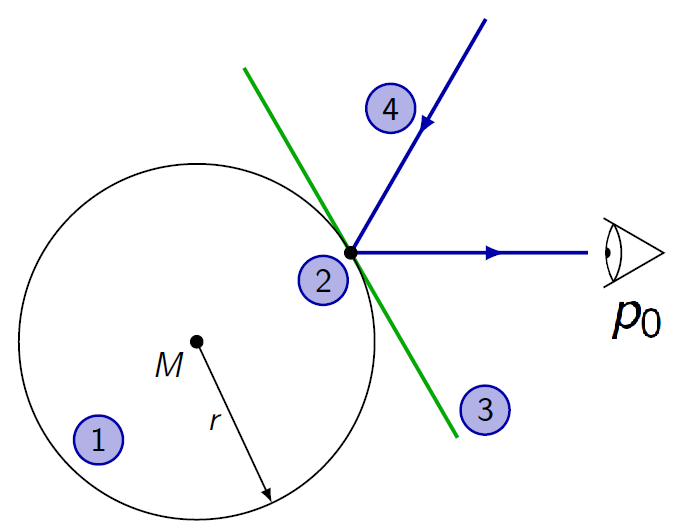
\includegraphics[width=\textwidth]{pics/Kugelprojektion.png}
	\end{minipage}
	\begin{minipage}{0.6\textwidth}
		\begin{enumerate}
			\item Gleichung für Kugel
			\item Durchstosspunkt
			\item Tangentialebene (Falls relevant)
			\item Reflektierter Strahl
		\end{enumerate}
	\end{minipage}\\
	\begin{enumerate}
		\item Kugelgleichung:
			\begin{equation*}
				(\vec{p} - \vec{m})\bullet (\vec{p} - \vec{m}) = r^2
			\end{equation*}
		\item Durchstosspunkt berechnen:\\
			Geradengleichung $\vec{p} = \vec{p_0} + s \cdot \vec{r}$ in Kugelgleichung einsetzen:\\
			\begin{tabular}{ll}
				$p_0 = $ Ortsvektor von Punkt $P_0$ & $\vec{r} = $ Richtungsvektor 
			\end{tabular}
			\begin{equation*}
			(\vec{p_0} + s \cdot \vec{r} - \vec{m})\bullet (\vec{p_0} + s \cdot \vec{r} - \vec{m}) = r^2
			\end{equation*}
			\begin{equation*}
			((\vec{p_0}-\vec{m}) + s \cdot \vec{r}) 
			\bullet
			((\vec{p_0}-\vec{m}) + s \cdot \vec{r}) = r^2
			\end{equation*}
			\begin{equation*}
			s^2 \cdot (\vec{r} \bullet \vec{r}) +
			s\cdot(2 \cdot (\vec{p_0}-\vec{m}) \bullet \vec{r}) +
			(\vec{p_0}-\vec{m}) \bullet (\vec{p_0}-\vec{m})
			-r^2 = 0
			\qquad \rightarrow \qquad
			s_{1/2} = \displaystyle \frac{-b \pm \sqrt{b^2-4ac}}{2a}
			\end{equation*}
			Es muss nun das kleinere  $s$ gewählt werden da mit diesem s der Durchstosspunkt welcher näher bei $P_0$ liegt gefunden wird.\\
			Nun muss der Punkt $P_1$ berechnet werden dazu muss $s$ in die Geradengleichung eingesetzt werden.
			\begin{equation*}
			\vec{p_1} = \vec{p_0} + s_1 \cdot \vec{r}
			\end{equation*}
						
		\item Reflektierter Strahl berechnen\\
		Zuerst muss der Normalenvektor der Tangentialebene bestimmt werden. Dieser geht von $P_1$ nach $M$ und hat die Länge $r$:\\
		\begin{equation*}
			\vec{n} = \vec{m} -\vec{p_1}
		\end{equation*}
		Nun muss der Richtungsvektor $\vec{r}$ in $\vec{r_\perp}$ und in $\vec{r_\parallel}$ aufgeteilt werden:\\
			\begin{minipage}{0.5\textwidth}
			\begin{equation*}
			\vec{r_\perp} = \displaystyle \frac{\vec{r} \bullet \vec{n}}{|\vec{n}|} \cdot
			\displaystyle \frac{\vec{n}}{|\vec{n}|}
			= \displaystyle \frac{\vec{r} \bullet \vec{n}}{r^2} \cdot \vec{n}
			\end{equation*}
			\begin{equation*}
			\vec{r_\parallel} = \vec{r} - \vec{r_\perp}
			\end{equation*}
			\begin{equation*}
			\vec{r'} = \vec{r_\parallel} - \vec{r_\perp} =
			\vec{r} - 2 \cdot \vec{r_\perp} =
			\vec{r} -2 \cdot \displaystyle \frac{\vec{r} \bullet \vec{n}}{r^2} \cdot \vec{n}
			\end{equation*}
			\end{minipage}
		\begin{minipage}{0.5\textwidth}
			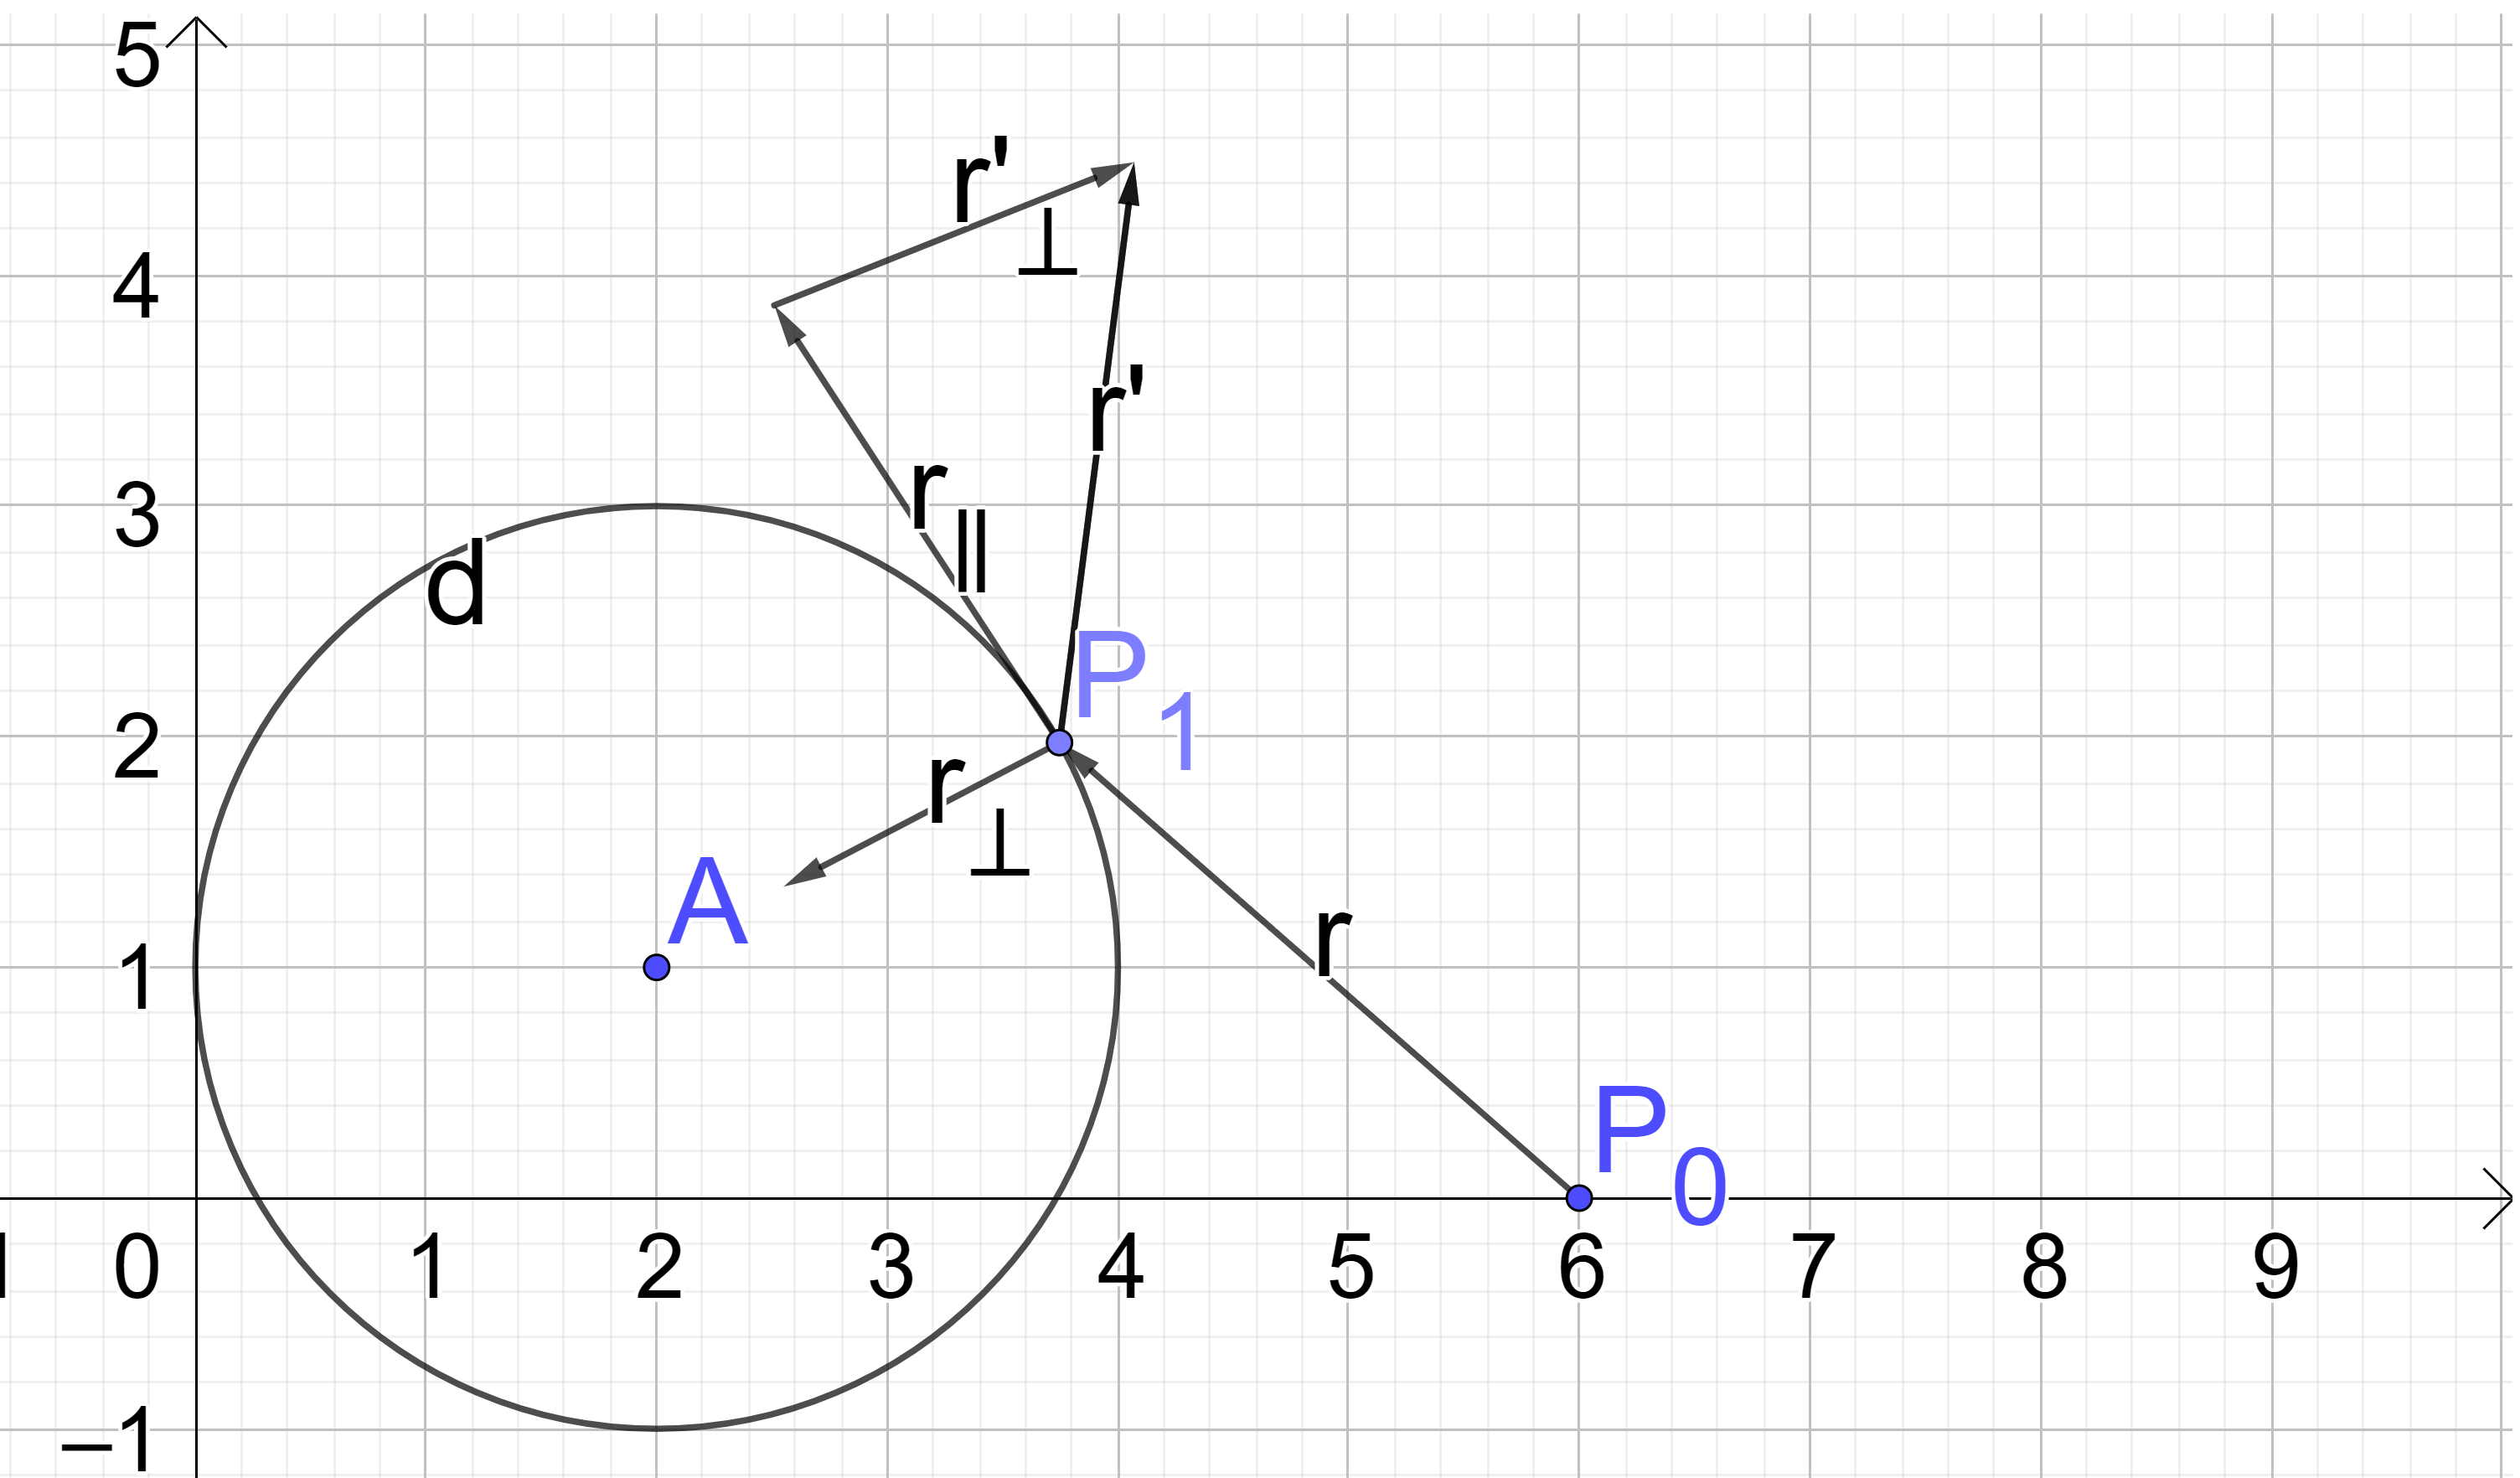
\includegraphics[width=\textwidth]{pics/Kugelprojektion_2.png}
		\end{minipage}
	
	\item Tangentialebene
		Wenn nun doch die Tangentialebene berechnet werden muss kann dies mit einer der folgenden Formeln gemacht werden
		\begin{itemize}
			\item $(\vec{p} - \vec{p_1}) \bullet (\vec{p_1} - \vec{m}) = 0 \qquad \qquad \vec{p} =$ Punkt auf Ebene
			\item $(\vec{p}-\vec{m}) \bullet (\vec{p_1} - \vec{m})=r^2$
		\end{itemize}
	\end{enumerate}

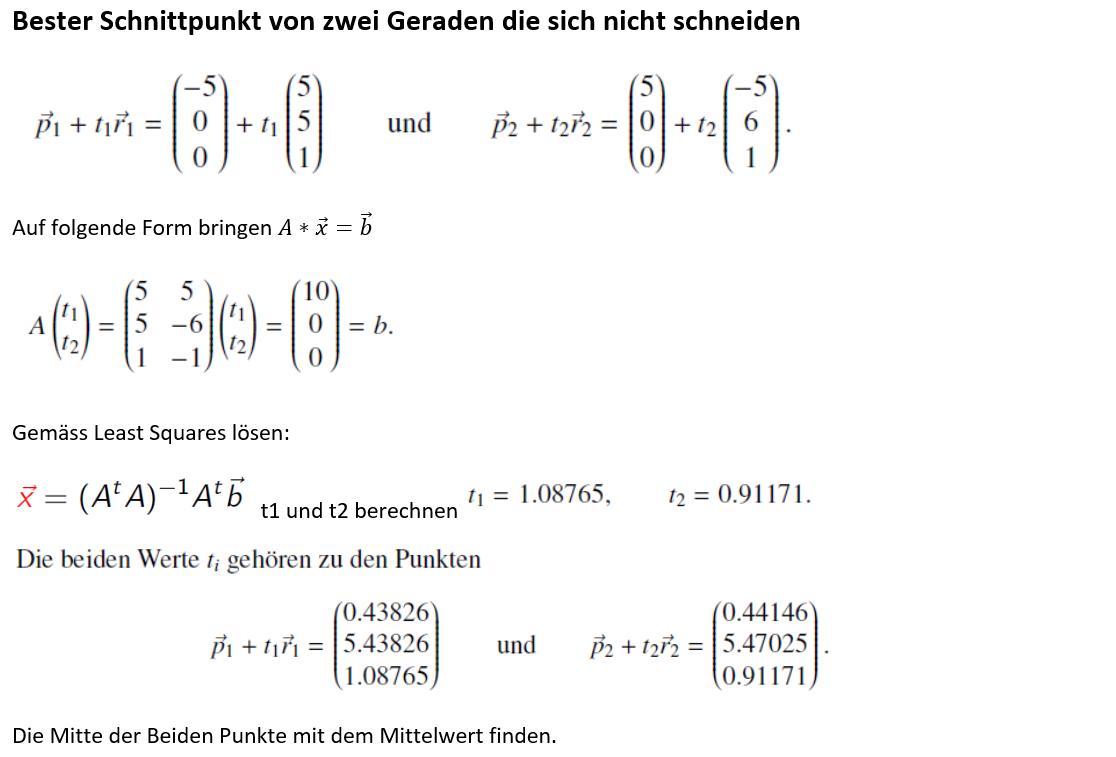
\includegraphics[width=0.8\textwidth]{pics/bsp_1.png}\\
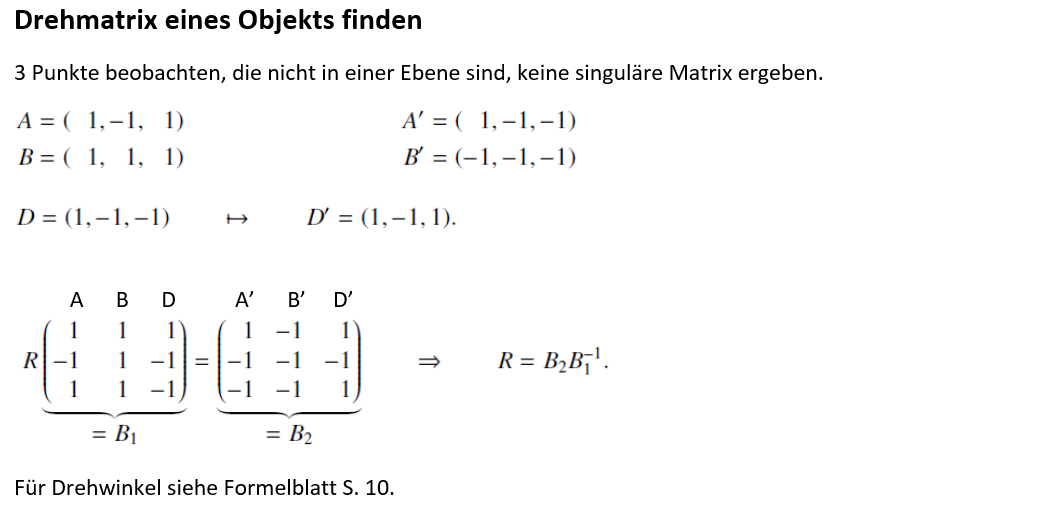
\includegraphics[width=0.8\textwidth]{pics/bsp_2.png}\\
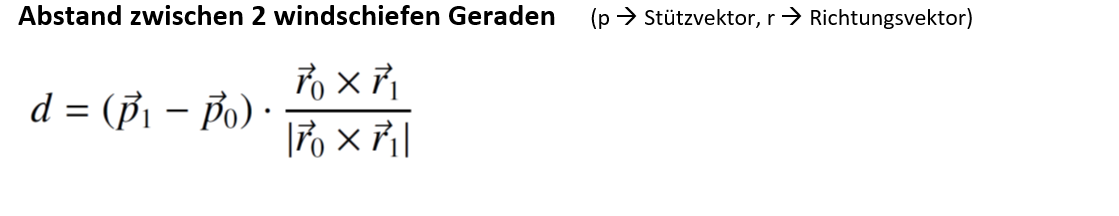
\includegraphics[width=0.6\textwidth]{pics/bsp_3.png}\\
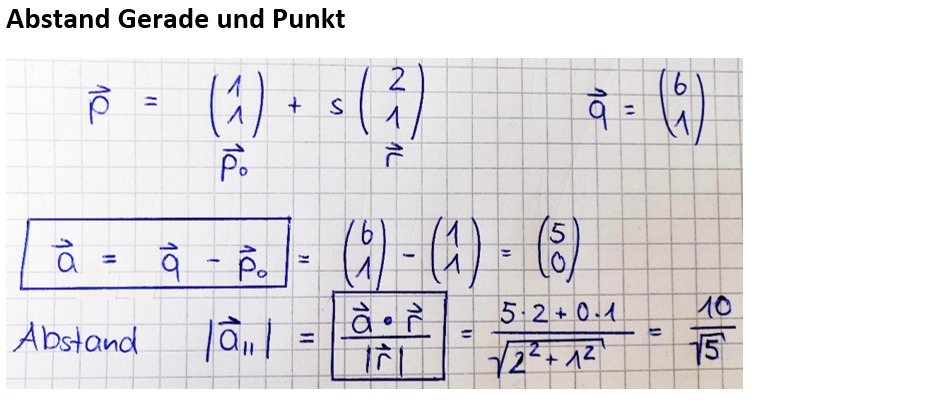
\includegraphics[width=0.6\textwidth]{pics/bsp_4.png}\\
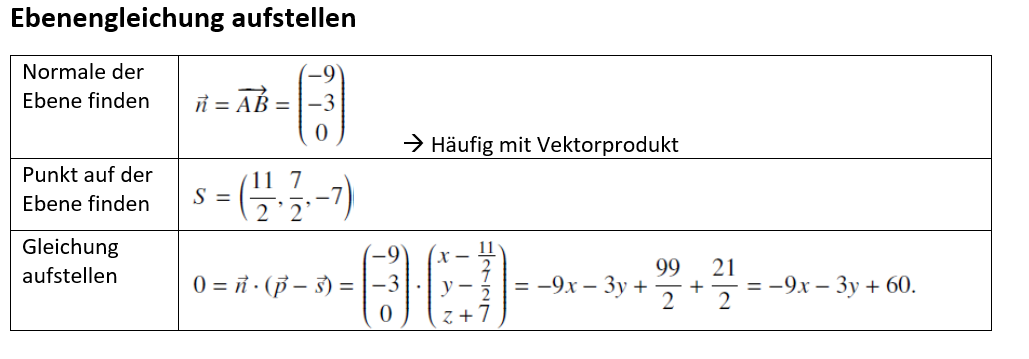
\includegraphics[width=0.8\textwidth]{pics/bsp_5.png}\\
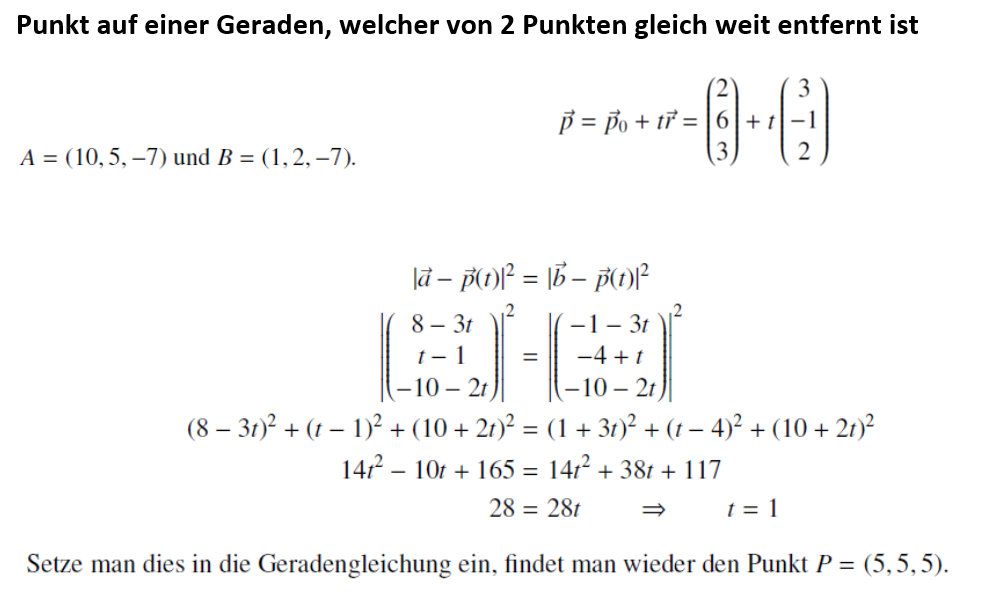
\includegraphics[width=0.8\textwidth]{pics/bsp_6.png}\\
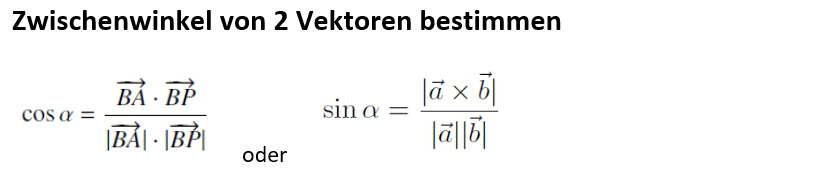
\includegraphics[width=0.6\textwidth]{pics/bsp_7.png}\\
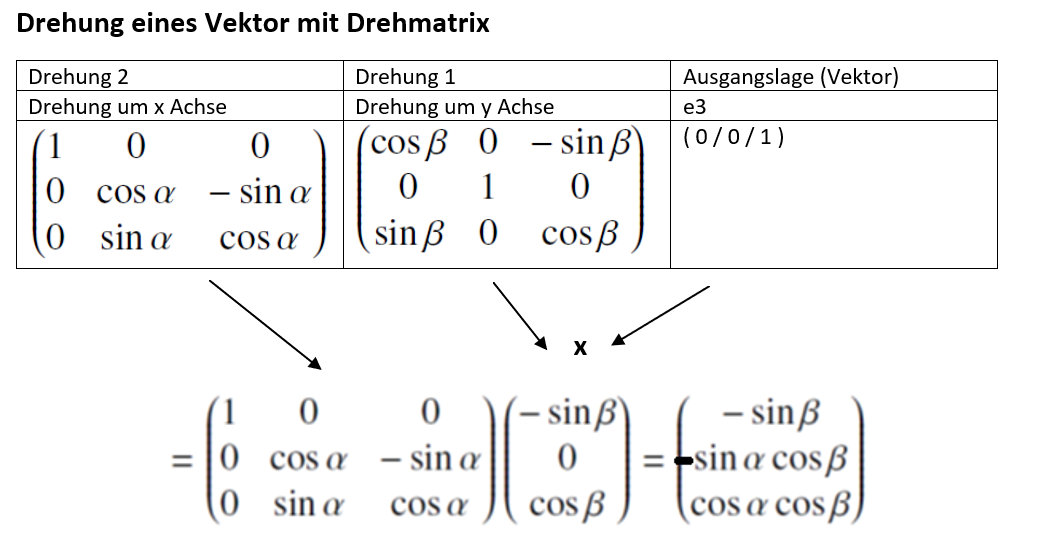
\includegraphics[width=0.8\textwidth]{pics/bsp_8.png}\\
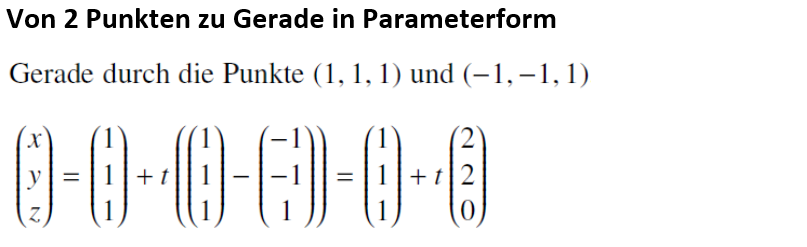
\includegraphics[width=0.6\textwidth]{pics/bsp_9.png}\\
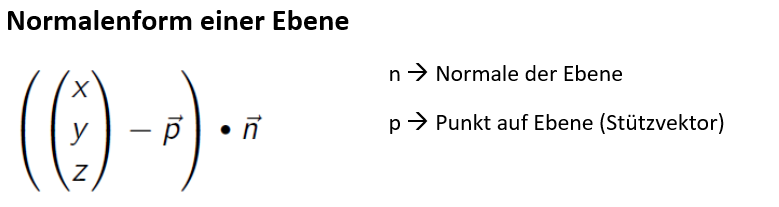
\includegraphics[width=0.6\textwidth]{pics/bsp_10.png}\\
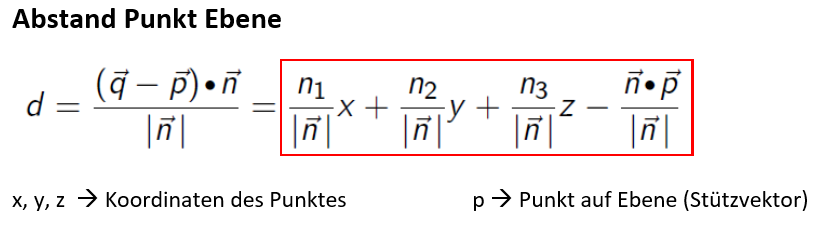
\includegraphics[width=0.6\textwidth]{pics/bsp_11.png}\\
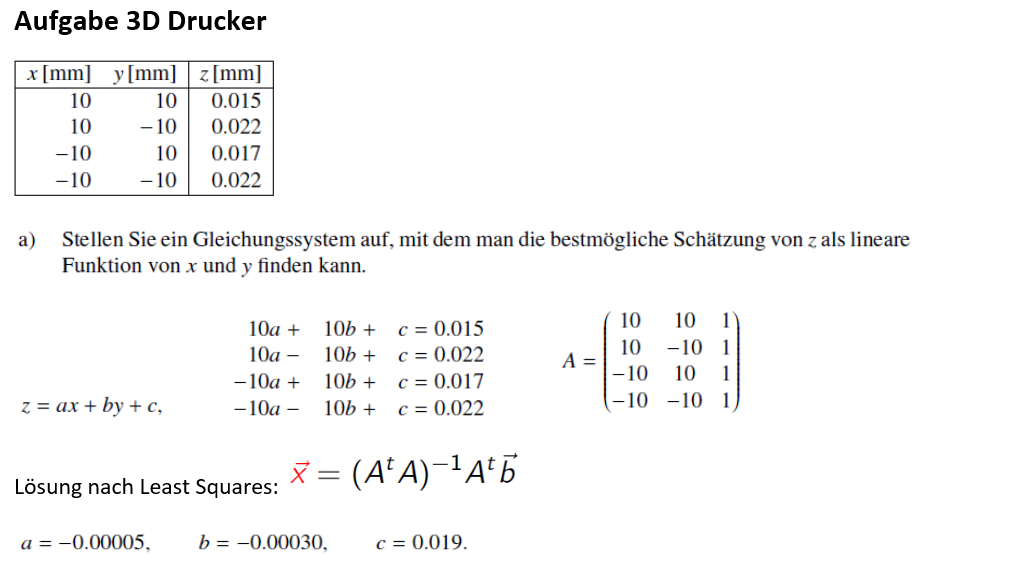
\includegraphics[width=0.8\textwidth]{pics/bsp_12.png}

\clearpage
\begin{sidewaystable}
	\section{Tabelle spezieller Matrizen}
		\begin{equation*}
			\begin{tabular}{|p{3cm}|c|c|c|p{2cm}|p{3cm}|c|p{2cm}|}
				\hline
					Name & Matrix & Spur & det & Eigenwert(e) (EW(A)) & Charakteristisches Polynom & Inverse $(A^{-1})$ & Orthogonalit. \\
				\hline
					Einheitsmatrix & $E = \begin{bmatrix} 1 & 0 \\ 0 & 1 \end{bmatrix}$	& n (2) & 1 & 1 & $\lambda^2 -2 \lambda + 1$ & 
					$E^{-1} = E$ & Orthogonal \\
				\hline
					Punktspiegelung & $P = \begin{bmatrix} -1 & 0 \\ 0 & -1 \end{bmatrix}$ & n (-2) & 1 & -1 & $\lambda^2 +2 \lambda + 1$ & 
					$P^{-1} = P$ & Orthogonal \\
				\hline
					Streckung am Urspung um Faktor 1 & $Z_{\lambda} = Z_{3} = \begin{bmatrix} 3 & 0 \\ 0 & 3 \end{bmatrix} = \begin{bmatrix} \lambda & 0 \\ 0 & \lambda \end{bmatrix}$ & $\lambda n (2 \cdot 3)$ & $\lambda^n (3^2)$ & $\lambda$ & $\lambda \neq \lambda$ \endgraf $\lambda^2 -2 \lambda a + a^2$\endgraf $a = \lambda$ von vorher = Streckung! & \endgraf $Z_{a}^{-1} = \frac{1}{a} E$ & Nicht orthogonal \\
				\hline
					Projektion auf X-Achse & $P_{X} = \begin{bmatrix} 1 & 0 \\ 0 & 0 \end{bmatrix}$ & 1 & 0 & 0 \& 1 & $
					\lambda^2 - \lambda = \lambda (\lambda - 1)$ & Keine! & Nicht orthogonal \\
				\hline
					Projektion auf Y-Achse & $P_{Y} = \begin{bmatrix} 0 & 0 \\ 0 & 1 \end{bmatrix}$ & 1 & 0 & 0 \& 1 & $
					\lambda^2 - \lambda = \lambda (\lambda - 1)$ & Keine! & Nicht orthogonal \\
				\hline
					Spiegelung an X-Achse & $S_{X} = \begin{bmatrix} 1 & 0 \\ 0 & -1 \end{bmatrix}$ & 0 & -1 & 1 \& 1 & $
					\lambda^2 - \lambda = \lambda (\lambda - 1)$ & $S_{X} = S_{X}^{-1}$ & Orthogonal \\
				\hline
					Spiegelung an X-Achse & $S_{Y} = \begin{bmatrix} -1 & 0 \\ 0 & 1 \end{bmatrix}$ & 0 & -1 & -1 \& 1 & $
					\lambda^2 - \lambda = \lambda (\lambda - 1)$ & $S_{Y} = S_{Y}^{-1}$ & Orthogonal \\
				\hline
					Drehmatrix allgemein! & $R_{\alpha} = \begin{bmatrix} \cos{\alpha} & -\sin{\alpha} \\ \sin{\alpha} & \cos{\alpha} \end{bmatrix}$ & $2 \cos{\alpha}$ & 1 & 0 = Keine reelle Lösung! & $\lambda^2 + -2 \lambda \cos{\alpha} + 1$ & $R_{\alpha}^{-1} = \begin{bmatrix} \cos{\alpha} & \sin{\alpha} \\ -\sin{\alpha} & \cos{\alpha} \end{bmatrix}$ & Orthogonal \\
				\hline
					Drehung um X-Achse! & $R_{x}(\alpha) = \begin{bmatrix} 1 & 0 & 0 \\ 0 & \cos{\alpha} & -\sin{\alpha} \\ 
					0 & \sin{\alpha} & \cos{\alpha} \end{bmatrix}$ & $1 + 2 \cos{\alpha}$ & 1 & 0 & 
					$(\lambda - 1)(\lambda^2 - 2 \lambda \cos{\alpha} + 1)$ & $R_{x}(\alpha)^{-1} = \begin{bmatrix} 1 & 0 & 0 \\ 0 & \cos{\alpha} & \sin{\alpha} \\ 0 & -\sin{\alpha} & \cos{\alpha} \end{bmatrix}$ & Orthogonal \\
				\hline
					Drehung um Y-Achse! & $R_{y}(\alpha) = \begin{bmatrix} \cos{\alpha} & 0 & \sin{\alpha} \\ 
					0 & 1 & 0 \\ -\sin{\alpha} & 0 & \cos{\alpha} \end{bmatrix}$ & $1 + 2 \cos{\alpha}$ & 1 & 0 & 
					$(\lambda - 1)(-\lambda^2 + 2 \lambda \cos{\alpha} - 1)$ & $R_{y}(\alpha)^{-1} = \begin{bmatrix} \cos{\alpha} & 0 & -\sin{\alpha} \\ 0 & 1 & 0 \\ \sin{\alpha} & 0 & \cos{\alpha} \end{bmatrix}$ & Orthogonal \\
				\hline
					Drehung um Z-Achse! & $R_{z}(\alpha) = \begin{bmatrix} \cos{\alpha} & -\sin{\alpha} & 0 \\ 
					\sin{\alpha} & \cos{\alpha} & 0 \\ 0 & 0 & 1 \end{bmatrix}$ & $1 + 2 \cos{\alpha}$ & 1 & 0 & 
					$(\lambda - 1)(-\lambda^2 + 2 \lambda \cos{\alpha} - 1)$ & $R_{z}(\alpha)^{-1} = \begin{bmatrix} \cos{\alpha} & \sin{\alpha} & 0 \\ -\sin{\alpha} & \cos{\alpha} & 0 \\ 0 & 0 & 1 \end{bmatrix}$ & Orthogonal \\
				\hline
					Drehung um $\frac{\pi}{2}$ von Ursprung im GU8! & $R_{\frac{\pi}{2}} = \begin{bmatrix} 0 & -1 \\ 1 & 0 \end{bmatrix}$ 
					& 0 & 1 & 0 & $\lambda^2 + \lambda = \lambda (\lambda + 1)$ & $R_{\frac{\pi}{2}}^{-1} = \begin{bmatrix} 0 & 1 \\ -1 & 0 \end{bmatrix}$ & Orthogonal \\
				\hline
					Drehung um $-\frac{\pi}{2}$ von Ursprung im GUS! & $R_{-\frac{\pi}{2}} = \begin{bmatrix} 0 & 1 \\ -1 & 0 \end{bmatrix}$ & 0 & 1 & 0 & $\lambda^2 + \lambda = \lambda (\lambda + 1)$ & $R_{-\frac{\pi}{2}}^{-1} = \begin{bmatrix} 0 & -1 \\ 1 & 0 \end{bmatrix}$ & Orthogonal \\
				\hline
					Drehung um $\frac{\pi}{4}$ & $R_{\frac{\pi}{4}} = \frac{1}{\sqrt{2}} \begin{bmatrix} 1 & -1 \\ 1 & 1 \end{bmatrix}$ & $\sqrt{2}$ & 1 & 0 & $\lambda^2 -\sqrt{2} \lambda + 1$ & $R_{\frac{\pi}{4}}^{-1} = \frac{1}{\sqrt{2}} \begin{bmatrix} 1 & 1 \\ -1 & 1 \end{bmatrix}$ & Orthogonal \\
				\hline
					Nullmatrix & $0 = \begin{bmatrix} 0 & 0 \\ 0 & 0 \end{bmatrix}$	& 0 & 0 & 0 & $\lambda^n$ & Keine! & Nicht orthogonal \\
				\hline
			\end{tabular}
		\end{equation*}
\end{sidewaystable}


%\newpage
\clearpage
\kariert{50}
\clearpage
\section{TR-Bedienung}
Diese Anleitung ist für den \textbf{TI-Nspire CX CAS} Rechner.\\[0.4cm]
\begin{tabular}{ll}
	Matrizen \& Vektoren einfügen: & 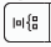
\includegraphics[height=0.6cm]{pics/TR_Symbol.png} $\rightarrow$ gewünschtes Element auswählen\\[0.2cm]
	Zeile an Matrix hinzufügen: & 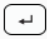
\includegraphics[height=0.6cm]{pics/TR_Enter_Pfeil.png}\\[0.2cm]
	Spalte an Matrix hinzufügen: & 
\includegraphics[height=0.6cm]{pics/TR_Shift.png} $\rightarrow$ 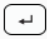
\includegraphics[height=0.6cm]{pics/TR_Enter_Pfeil.png}\\[0.8cm]
	
	Determinante: & det($[...]$) $\rightarrow$ 
\includegraphics[height=0.6cm]{pics/TR_Enter.png}\\[0.2cm]
	& oder\\[0.2cm]
	& 
\includegraphics[height=0.6cm]{pics/TR_Menu.png} $\rightarrow$ 7 $\rightarrow$ 3 $\rightarrow$ 
\includegraphics[height=0.6cm]{pics/TR_Enter.png}\\[0.2cm]
	Inverse: & $[...]^{-1} \rightarrow$ 
\includegraphics[height=0.6cm]{pics/TR_Enter.png}\\[0.2cm]
	Transponieren & $[...]$ 
\includegraphics[height=0.6cm]{pics/TR_Menu.png} $\rightarrow$ 7 $\rightarrow$ 2 $\rightarrow$ 
\includegraphics[height=0.6cm]{pics/TR_Enter.png}\\[0.2cm]
	Gauss ohne rückw. einsetzen: & ref($[...]$) $\rightarrow$ 
\includegraphics[height=0.6cm]{pics/TR_Enter.png}\\[0.2cm]
	Gauss: & rref($[...]$) $\rightarrow$ 
\includegraphics[height=0.6cm]{pics/TR_Enter.png}\\[0.2cm]
	Gauss Schritte ohne Rückw.\footnotemark[1]: & linalgcas\textbackslash gausstep($[...]$) $\rightarrow$ 
\includegraphics[height=0.6cm]{pics/TR_Enter.png}\\[0.2cm]
	Inverse Schritte\footnotemark[1]: & linalgcas\textbackslash inversestep($[...]$) $\rightarrow$ 
\includegraphics[height=0.6cm]{pics/TR_Enter.png}\\[0.8cm]
	
	Kreuzprodukt: & crossP([X,Y,Z],[X,Y,Z])\\[0.2cm]
	Skalarprodukt: & dotP([X,Y,Z],[X,Y,Z])\\[0.2cm]
	Betrag: & norm([X, Y, Z])\\[0.8cm]
	
	Eigenwerte: & cPolyRoots($r^2 + 2r + 1$, $r$)\\[0.2cm]

\end{tabular}
\footnotetext[1]{Nur wenn LinAlgCAS Library vorhanden ist.}

\end{document}